%For arxiv submission
\documentclass[useAMS, usenatbib]{mnras}
\usepackage{graphicx,amsmath,color,amssymb}
%\voffset=-0.8in
%MNRAS
%\documentclass[useAMS, usenatbib, usegraphicx, twocolumn]{mnras}

%[YAH commented out, my editor didn't like it...]
\usepackage[pdftitle={A hybrid particle-analytic method for non-linear neutrino structure}]{hyperref}

% \newcommand{\eprint}[1]{\href{http://arxiv.org/abs/#1}{#1}}
% \newcommand{\adsurl}[1]{\href{#1}{ADS}}


\topmargin -1.5cm
\bibliographystyle{mnras}

\newcommand{\beq}{\begin{equation}}
\newcommand{\eeq}{\end{equation}}
\newcommand{\barr}{\begin{eqnarray}}
\newcommand{\earr}{\end{eqnarray}}

\newcommand{\rme}{\textrm{e}}
\newcommand{\rmH}{\textrm{H}}
\newcommand{\Ly}{\textrm{Ly}}
\newcommand{\pabn}{p_{\textrm{ab}}^n}
\newcommand{\pscn}{p_{\textrm{sc}}^n}
\newcommand{\rmd}{\textrm{d}}
\newcommand{\N}{\mathcal{N}}
\newcommand{\nuc}{\nu_{\rm c}}
\newcommand{\Tm}{T_{\rm m}}
\newcommand{\Tr}{T_{\rm r}}
\newcommand{\nh}{n_{\rm H}}
\newcommand{\bfA}{\boldsymbol{A}}
\newcommand{\bfr}{\boldsymbol{r}}
\newcommand{\bfV}{\boldsymbol{V}}
\newcommand{\bs}{\mathbf}
\newcommand{\mH}{\mathcal{H}}

\newcommand{\natu}{Nature (London)}
\newcommand{\aas}{Bull. Am. Astron. Soc.}
\newcommand{\gadget}{{\small GADGET\,}}

\newcommand{\spb}[1]{{\textcolor{green}{[{\bf SPB}: #1]}}}
\newcommand{\yah}[1]{{\textcolor{red}{[{\bf YAH}: #1]}}}

\newcommand{\Mpch}{\,\mathrm{Mpc} \,h^{-1}}
\newcommand{\hMpc}{h^{-1}\,\mathrm{Mpc}}
\newcommand{\Lya}{Lyman-$\alpha\;$}
%%%%%%%%%%%%%%%%%%%%%%%%%%%%%%%%%%%%%%%%%%%%%%%%%%%%%%%%%%%%%%%%%%%%%%%%%%%%%%%%%%%%%%%%%%%%%%%%%%


\begin{document}

\title{A Hybrid Method for Simulating Non-Linear Neutrino Structure}
%\title{Converged Simulations for Non-Linear Neutrino Structure Using a Hybrid Method}
\author[ S. Bird et al.]{  Simeon Bird$^1$\thanks{E-mail: sbird@ucr.edu}, Yacine Ali-Ha\"{\i}moud$^2$, Yu Feng$^3$, Jia Liu$^4$\vspace{1.5mm}\\
$^1$Institution\\
$^2$Center for Cosmology and Particle Physics, Department of Physics,
New York University, New York, NY 10003, USA\\
$^3$Institution\\
$^4$Institution}

\date{\today}

\pagerange{\pageref{firstpage}--\pageref{lastpage}} \pubyear{2012}
\pagenumbering{arabic}
\label{firstpage}

\maketitle

\begin{abstract}
\yah{I would present this paper as a ``proof of concept" for the hybrid method, and defer a thorough convergence test to future work (as a referee, I would definitely ask us to do more quantitative tests). Unless of course it is easy to do more tests :-)}

\end{abstract}

\begin{keywords}
        neutrinos - cosmology: large-scale structure of Universe - cosmology: dark matter
\end{keywords}

\section{Introduction}

\spb{3. Change vcrit to 850. 5. Implement numerical derivative of CAMB transfer in MP-GenIC.}

%Cite bahamas and Liu. Cite any other major simulation projects that used the neutrino code.

%Neutrinos have mass. Neutrino mass is important because. Neutrinos affect structure. In order to measure the mass accurately with structure we need to know precisely how neutrinos affect structure.
%The structure in question is non-linear structure. We thus need to run simulations. This paper is about a method to put neutrinos into structure simulations.
Neutrinos are the lightest standard model particles, and neutrino oscillation experiments have shown that the sum of the neutrino masses is $M_\nu > 0.06$ eV \citep{Becker-Szendy_1992, Fukuda_1998}.
However, measuring the neutrino mass in the laboratory is challenging due to the large difference in mass scales between neutrinos and other standard model particles \cite[although see][]{Wolf_2010}.

However, massive neutrinos in the cosmic neutrino background also affect the growth of large scale structure.
Massive neutrinos behave as light thermal relics, suppressing clustering below their thermal
free-streaming length \citep[e.g.][]{Lesgourgues_2006, Wong_2011}.
Measurements of the clustering of matter and matter tracers in the Universe can detect this effect and thus constrain the total mass of neutrinos.

Cosmological constraints on the neutrino mass sum ($M_\nu$) are quickly approaching the lower limit implied by neutrino oscillation data. For example, the Planck team obtained a 95 \% CL upper limit of $M_\nu<0.23$~eV~\citep{planck2015xiii} using primary cosmic microwave background (CMB) temperature data, combined with low-$\ell$ polarization, CMB lensing, type Ia supernovae~\citep{Betoule_2014}, and baryon acoustic oscillation
measurements~\citep{Beutler_2011, Anderson_2014, Ross_2015}. \cite{Palanque_2015} found a tighter constraint of $M_\nu<0.15$~eV by adding Lyman-$\alpha$ forest data from the Sloan Digital Sky Survey (SDSS). However, recent weak lensing data from the Dark Energy Survey combined with Planck weakens the upper limit to $0.29$ eV \citep{DES_2017}, and the most recent galaxy power spectrum measurements from SDSS show a slight preference for a non-zero neutrino mass of $M_\nu = 0.3$ eV \citep{Beutler_2014}.
%Not citing HSC or KIDS because they are not yet competitive neutrino mass constraints \citep{HSC_2017}.
% Taken together, these experiments indicate that a detection of neutrino mass from cosmology is imminent. However, realizing the statistical power of future surveys will require extremely accurate modelling
%of structure growth.
Near-future large cosmological surveys such as the Dark Energy Spectroscopic Instrument (DESI) \citep{DESI} or the
Large Synoptic Survey Telescope~(LSST) \citep{LSST, Joudaki_2012} will have the statistical power to measure the neutrino mass even if it is close to $0.06$ eV, the minimum required by oscillation experiments \citep{Abazajian_2015}.

Realizing the statistical power of future surveys will require extremely accurate modelling of structure growth and the effects of massive neutrinos on the matter density field.
Furthermore, current and future experiments achieve their statistical power from small scales where structure formation is in the non-linear regime \citep[e.g.~][]{Troxel_2017, HSC_2017}.
As following structure growth on non-linear scales ultimately requires fitting to $N$-body cosmological simulations, there is an urgent need to incorporate massive neutrinos into cosmological structure simulations
in a way both accurate and computationally inexpensive.
If the simulation methods used are insufficiently accurate, experiments will measure incorrect values for the neutrino mass.
Conversely, if simulation techniques are overly computationally intensive, the number of simulations which can be performed will be reduced, again impeding the accuracy of the cosmological parameter measurement.

\cite{AHB}, hereafter AHB13, proposed modelling neutrinos using a perturbative linear response approximation \citep{Bond_1980, Ma_1994}, described in more detail in Section~\ref{sec:analytic}. The neutrino component is followed using first-order linear perturbation theory, clustering in a background potential generated from the fully non-linear clustering of the CDM particles. The main improvement of this method over earlier perturbation-based neutrino codes \citep{Brandbyge_2009} was the use of the full non-linear CDM potential. This makes it possible to achieve accurate results for any level of CDM clustering, as long as the neutrino free-streaming scale is larger than the non-linear scale.
The linear-response method is computationally efficient and accurately describes the effect of massive neutrinos on the growth of cold dark matter (CDM), computing the matter power spectrum $P(k)$ at around $1\%$ accuracy for $M_\nu \lesssim 0.6$ eV.
Due to its minimal computational overhead,
it has been used to investigate the combined effects of massive neutrinos and baryons \citep{Mummery_2017} and to constrain the neutrino mass using hydrodynamic simulations of large-scale structure \citep{McCarthy_2018, McCarthy_2017}.

However, AHB13 found that this method did not reproduce the growth of the neutrino power seen in particle simulations for $M_\nu > 0.3$ eV  and $z < 0.5$, even though the expected over-density remained less than unity. The linear response method becomes inaccurate when collisionless particles have a slow initial velocity. As the initial velocity of neutrinos follows a Fermi-Dirac distribution, there are massive neutrinos whose velocities are low enough to cluster non-linearly. These neutrinos can dominate the clustering on small scales, even if they are a small fraction of the neutrino matter density, because linear growth is highly suppressed. \spb{Does the above rephrasing work for you?}

In this paper, we present an extension of the linear-response method which allows to accurately model neutrinos with low initial velocities, and thus reproduce the neutrino power spectrum from particle simulations. The neutrinos are split into two fast and slow components by their initial velocity. The slow component is followed using neutrino particles while the fast component is followed using the linear response approximation.  Note that the slow initial velocity of our particle neutrinos mitigates the numerical problems that plague purely particle simulations. Our new method allows, for the first time, a single simulation code to produce a well-converged neutrino simulation, at any neutrino mass, which includes late-time non-linear growth in the neutrino sector. We describe it in more detail in Section~\ref{sec:hybrid}.

We provide an improved public implementation of our neutrino simulation
method\footnote{The latest version may be found here: \url{https://github.com/sbird/kspace-neutrinos/}}.
While the implementation in AHB13 was tied to \gadget \citep{Springel_2005}, our new version is adaptable to a variety of structure simulation codes. We also include patches for Gadget-2 \citep{Springel_2005}, which were used for a large suite of simulations in \cite{Liu_2017}.

In Section \ref{sec:methods}, we describe the different methods we have implemented to simulate neutrinos. We describe our
results and compare them against other methods in Section \ref{sec:results}. We conclude in Section \ref{sec:conclusion}. Appendix \ref{sec:manual} is a user's manual for our neutrino module and in Appendix \ref{sec:initcond} we describe improvements to our initial conditions since AHB13.

\section{Methods}
\label{sec:methods}

In this Section we describe our simulation techniques. Section~\ref{sec:particle} describes our implementation of particle neutrinos, the earliest and most widely used neutrino simulation method. Section \ref{sec:analytic} reviews the linear-response approximation. Section \ref{sec:hybrid} describes our hybrid technique, which builds on both earlier methods. Finally, Section~\ref{sec:simulations} details the parameters of our simulations.

\subsection{Particle Neutrinos}
\label{sec:particle}

The simplest method of simulating massive neutrinos is to model their phase-space distribution with discrete numerical ``particles", akin to the CDM, but with a lower particle mass and a large thermal velocity imposed
in the initial conditions. As for CDM, neutrino particles are given displacements and velocities using the Zel'dovich approximation \citep{Zeldovich_1970}, such that their initial power spectrum matches the linear transfer function. \footnote{For astrophysically relevant redshifts and neutrino masses, the neutrino velocity is completely dominated by their thermal velocities. We have verified explicitly that omitting the structure formation component of the initial neutrino velocities has negligible effect on the final result of the simulations.}

This approach has been used extensively in the past, in, e.g.~\cite{Brandbyge_2008, Bird_2012, Inman_2017, FVN_2017}. Its main advantages are that it is simple to implement and fully includes the non-linear physics of the
neutrinos\footnote{Although note that the small-scale tree force for the neutrino particles is often disabled in the literature.}. It has been used to examine voids \citep{Massara_2015}, clusters and halos \citep{FVN_2014, Castorina_2014, Costanzi_2013}, large-scale clustering \citep{Castorina_2015} and the ISW effect \citep{Carbone_2016}.
However, this method is computationally expensive and can suffer from a variety of numerical problems related to the large thermal velocities required by the neutrino particles.

For example, the discrete nature of the neutrino particles, and their random distribution, induces shot noise power $P \propto 1/N_\mathrm{part}$ at early times, which can only be reduced by a large particle load. In a parallel code the large thermal velocities of the neutrinos causes particles to frequently move between processors, limiting scalability. Furthermore, the particle approximation limits the physics that can be implemented. Modelling the splitting between neutrino mass states involves the use of at least two particle species.

Our implementation of particle neutrinos includes several novel features improving accuracy. The size of the long-range particle-mesh timestep in Gadget is chosen so that no particle moves more than a fraction of a grid cell in a single timestep. As in earlier work, we exempt the neutrinos from this constraint, lest the PM timestep become extremely small. However, unlike earlier work, we do self-consistently compute the timesteps of neutrinos for the short range tree force.

In earlier works \citep{Bird_2012}, we disabled the short-range tree force for the neutrino particles, leaving them affected only by the long-range particle-mesh force. Since the purpose of this work is to follow the non-linear small-scale evolution of the neutrinos accurately, we enable the short-range tree force in this work, although we use a softening length
twice that of the CDM particles, at $1/15$ th of the mean inter-particle spacing (which is still substantially smaller than the neutrino free-streaming length). This larger softening length was implemented initially to ensure that the smallest timesteps are not populated exclusively by neutrino particles, although we found in practice that it made little difference to simulation runtime or results.

The large velocity of the neutrino particles caused severe numerical issues in Gadget-3, manifesting as frequent hangs when walking the short-range gravitational force tree. We traced these problems to an optimisation present in Gadget-3. In order to avoid the overhead of regenerating the force tree every timestep, the tree persists over short timesteps. Particle motion is accounted for by moving tree nodes according to the average velocity of particles within each node. Neutrino particles have large random thermal velocities, which cause them to frequently move from one force node to another. It is thus not sufficient to account for particle motion by moving the node of the force tree, and one must instead perform a full rebuild of the force tree on every timestep. We found that a more frequent rebuilding of the force tree improves the accuracy of the simulation even without neutrino particles, and thus we have made rebuilding the force tree each timestep the default behaviour in MP-Gadget. We implemented a number of optimizations in the tree build code to avoid it dominating the cost of the simulation.

%\subsection{Analytic Neutrinos}
%\label{sec:analytic}
%
%
%In this section we describe the semi-analytic linear response method for treating neutrinos from \cite{AHB}.
%Motivated by the numerical difficulties with particle simulations, we sought to use an analytic treatment.
%The applicability of this method follows is because neutrinos do not cluster below their free-streaming length, given by
%\begin{equation}
% k_{\rm fs}(z) \approx \frac{0.08}{\sqrt{1+z}}
%\sqrt{\frac{\Omega_{\rm M}}{0.3}} \frac{m_{\nu}}{0.1 ~ \textrm{eV}} h~ \textrm{Mpc}^{-1}.
%\label{eq:kfs}
%\end{equation}
%For astrophysically relevant neutrino masses, this free-streaming length is larger than the non-linear scale.
%Thus while CDM exhibits strong non-linear clustering, the neutrino species does not, behaving
%almost as expected from linear perturbation theory. However, the neutrino species does exhibit increased clustering
%as a result of the deeper non-linear CDM potential. The method of \cite{AHB} is thus a linear response,
%in which the neutrino linear theory perturbation grows due as a result of the non-linear growth of CDM.
%
%The neutrino power-spectrum is then given by (eq. (63) of \cite{AHB})
%\begin{align}
%P_{\nu}^{1/2}(k, \tau) &= \mathcal{I}_{s_i, s}
%P_{\nu}^{1/2}(k, \tau_i) \left\{1 - (s - s_i)  a_i [\theta_{\nu}/\delta_{\nu}]_{i}(k)\right\}\nonumber\\
%&+ \frac32 \Omega_{\rm M} H_0^2 \int_{\tau_i}^{\tau} \mathcal{I}_{s', s}
%P^{1/2}_{\rm M}(k, \tau') (s - s')d \tau', \label{eq:P-final}
%\end{align}
%where $\mathcal{I}_{s_1, s_2} \equiv \mathcal{I}([s_2 -s_1]k/m)$. $\mathcal{I}$ is defined to be
%the Fourier transform of the unperturbed neutrino distribution function in momentum space, normalized so
%that $\mathcal{I}(0) = 1$ \citep{Brandenberger_1987, Bertschinger_Watts_1988},
%\begin{equation}
%\mathcal{I}[X; f_0] \equiv \frac{\int dq~ j_0(q X) q^2 f_0(q) }{\int dq ~q^2 f_0(q)}. \label{eq:I.def}
%\end{equation}
%
%The first term of Eq.~\ref{eq:P-final} represents a contribution from the initial conditions. In practice
%for astrophysical masses neutrinos are initially relativistic, so this term is extremely small and may
%be safely neglected (although we include it in our implementation for completeness).
%The second term is the perturbation to a neutrino geodesic from the CDM potential
%integrated over cosmic time. Our implementation computes the matter power spectrum for every PM timestep
%and stores it in a table, evenly spaced in $\Delta a = 0.01$\footnote{The code actually provides the CDM power spectrum.
%We estimate the matter power spectrum by adding the neutrino power from the previous timestep. It would be possible
%to iterate this procedure, but in practice it is always immediately converged to a high degree of accuracy.}.
%The neutrino power spectrum is computed by performing an integral over all past matter power spectra, interpolated in log space.
%
%Eq.~\ref{eq:P-final} computes the neutrino power spectrum from stored CDM power spectra.
%A computation of the neutrino potential would use the CDM potential over all of cosmic history, which is impractical
%to store at the required number of time slices. We make the approximation that neutrinos and
%have a cross-correlation coefficient of unity. Thus, in order to recover the neutrino potential, we use
%\begin{equation}
%\delta_{\nu}(\bs k, \tau) = \left(\frac{P_{\nu}(k,
%    \tau)}{P_{\rm cdm}(k, \tau)}\right)^{1/2} \delta_{\rm cdm}(\bs k, \tau).\label{eq:phases}
%\end{equation}
%Equivalently, we assume that the neutrinos and CDM have identical Fourier phases or that neutrinos perfectly trace CDM structure.
%Physically, this is plausible: neutrinos behave much like CDM on scales larger than their free streaming length,
%and do not cluster on smaller scales (so any differences in their phases has limited practical impact, as $\delta_\nu$ is zero).
%Figure~\ref{fig:cross-corr} shows the cross-correlation coefficient,
%\begin{equation}
%R = \frac{\left\langle \delta_\nu \delta_\mathrm{cdm} \right\rangle}{\sqrt{P_{\rm{cdm}} P_{\rm{\nu}}}}
%\end{equation}
%between neutrinos and CDM from a neutrino particle simulation. It is indeed unity on large scales,
%dropping to zero on small scales where the particle neutrino power is dominated by shot noise.
%

\subsection{Linear-response approximation} \label{sec:analytic}

AHB13, motivated by numerical difficulties with particle simulations,
devised an analytic, linear response approximation. The central idea
is to solve the linearized collisionless Boltzmann equation for neutrinos,
using the full non-linear Newtonian potential of the cold dark matter.
In this section we briefly review the linear-response approximation,
for a general collisionless species with phase-space density $f$.

We denote by $s$ the ``superconformal" or ``Newtonian" time $(ds \equiv dt/a^2$, where $a$ is the scale factor), and overdots denote derivatives with respect to $s$. Comoving scales are denoted by $\bs{x}$ and $\bs{u} \equiv \dot{\bs{x}}$ denotes the rescaled peculiar velocity of a massive particle. We normalize the phase-space density such that the overdensity is given by
\beq
1 + \delta(s, \bs{x}) = \int d^3 u ~ f(s, \bs{x}, \bs{u}).
\eeq
For a non-relativistic particle, the geodesic equation is $\dot{\bs{u}} = - a^2  \bs{\nabla}_{\bs{x}} \phi$, where $\phi$ is the Newtonian potential. The phase-space density is conserved along trajectories, as is encoded by the collisionless Boltzmann (or Vlasov) equation
\beq
\dot{f} + \bs{u} \cdot \bs{\nabla}_{\bs{x}} f - a^2 \bs{\nabla}_{\bs{x}} \phi \cdot \bs{\nabla}_{\bs{u}} f = 0. \label{eq:Vlasov}
\eeq
The particle or $N$-body method solves the Vlasov equation numerically by effectively discretizing $f$. The linear-response method consists in solving for $f$ to linear order in the gravitational potential. Specifically, it is the first order in an expansion in the small parameter $\epsilon \sim a^2 \phi/u^2$. Such an expansion works increasingly well for fast or hot particles (and conversely, it is not adapted for cold particles, see \citealt{YAH_15}). We denote by $f_0(u)$ the unperturbed, homogenous and isotropic phase-space density, which integrates to unity. Fourier-transforming Eq.~\eqref{eq:Vlasov} and linearizing it, we get
\beq
\dot{f} + i (\bs{k} \cdot \bs{u}) f = i (\bs{k} \cdot  \hat{u}) \frac{d f_0}{du} a^2 \phi ,  \ \ \ \ \ \ \hat{u} \equiv \bs{u}/u.
\eeq
Given initial conditions at $s_i$, this has an explicit integral solution,
\barr
f(s, \bs{k}, \bs{u}) &=& \rme^{- (\bs{k} \cdot \bs{u}) (s - s_i)} f(s_i, \bs{k}, \bs{u}) \nonumber\\
&+& i (\bs{k} \cdot  \hat{u}) \frac{d f_0}{du} \int_{s_i}^s d s' \rme^{- i(\bs{k} \cdot \bs{u}) (s - s')} a'^2 \phi(s', \bs{k}).~~~
\earr
The overdensity is then obtained by integrating over velocities. Using Poisson's equation, $k^2 \phi = - \frac32 H_0^2 \Omega_M a^{-1} \delta_M$, where $\delta_M$ is the total matter overdensity, we arrive at
\barr
\delta(s, \bs{k}) &=& \int d^3 u ~ \rme^{- (\bs{k} \cdot \bs{u}) (s - s_i)} f(s_i, \bs{k}, \bs{u}) \nonumber\\
&+& \frac32 H_0^2 \Omega_M \int_{s_i}^s d s' (s-s') \mathcal{I}[k(s-s')] a' \delta_M(s', \bs{k}), ~~~~\label{eq:delta-phi}
\earr
where the kernel $\mathcal{I}$ is given by \citep{Brandenberger_1987, Bertschinger_Watts_1988}
\barr
\mathcal{I}(k \Delta s) &\equiv& - \frac{i}{k \Delta s} \int d^3 u  ~(\hat{k} \cdot  \hat{u}) \frac{d f_0}{du}\rme^{- i(\bs{k} \cdot \bs{u}) \Delta s} \nonumber\\
%&=& - \frac{1}{k \Delta s} \int d^3 u  \frac{d f_0}{du} j_1(u k \Delta s) \nonumber\\
&=& \int d^3 u ~	 j_0(u k \Delta s) f_0(u),
\earr
where in the last line we have integrated by parts, and $j_0(x) \equiv \sin x/x$ is the zero-th spherical Bessel function.

The first piece in Eq.~\eqref{eq:delta-phi} corresponds to the free propagation of initial perturbations between times $s_i$ and $s$. The second piece corresponds to the sourcing of perturbations by gravitational potentials. We have checked explicitly that the former is negligible relative to the latter for the problem at hand.
%, and we shall drop it in what follows. We do not actually drop it


Since we cannot afford to store the full three-dimensional matter density field as a function of time, we must simplify Eq.~\eqref{eq:delta-phi} further. Following AHB13, we approximate
\begin{equation}
 \delta_M(s', \bs{k}) \approx \sqrt{P_M(s', k)/P_M(s, k)}~ \delta_M(s, \bs{k})\,,
 \label{eq:phases}
\end{equation}
in the integral. This approximation is a priori only accurate on linear scales. However, as argued in AHB13, the non-linear scale is smaller than the free-streaming scale, which implies that on non-linear scales the kernel $\mathcal{I}$ suppresses early-time contributions to the integral. As a consequence, this approximation ought to be reasonably accurate on all scales. We can confirm this expectation using a particle neutrino simulation. Eq.~\ref{eq:phases} is equivalent to assuming that the cross-correlation between neutrinos and CDM is unity. Figure \ref{fig:cross-corr} shows the cross-correlation coefficient between neutrino particles and CDM in a particle simulation and in our new hybrid method, demonstrating that it is indeed close to unity as long as the neutrino power spectrum is not dominated by particle shot noise. This validates our use of Eq.~\ref{eq:phases}.

The approximation in Eq.~\ref{eq:phases} allows us to only store the one-dimensional matter power spectrum as a function of time\footnote{The code actually provides the CDM power spectrum. We estimate the matter power spectrum by adding the neutrino power from the previous timestep. It would be possible to iterate this procedure, but in practice it is always immediately converged to a high degree of accuracy, see Appendix B of AHB13.} We do so at even intervals $\Delta a = 0.01$. The neutrino power spectrum is computed by performing an integral over an interpolation of all past matter power spectra. \yah{Why log-space interpolation since stored on a linearly-spaced table in $a$?} \spb{I meant log(P(k)) is interpolated linearly in a, sorry.}

\begin{figure}
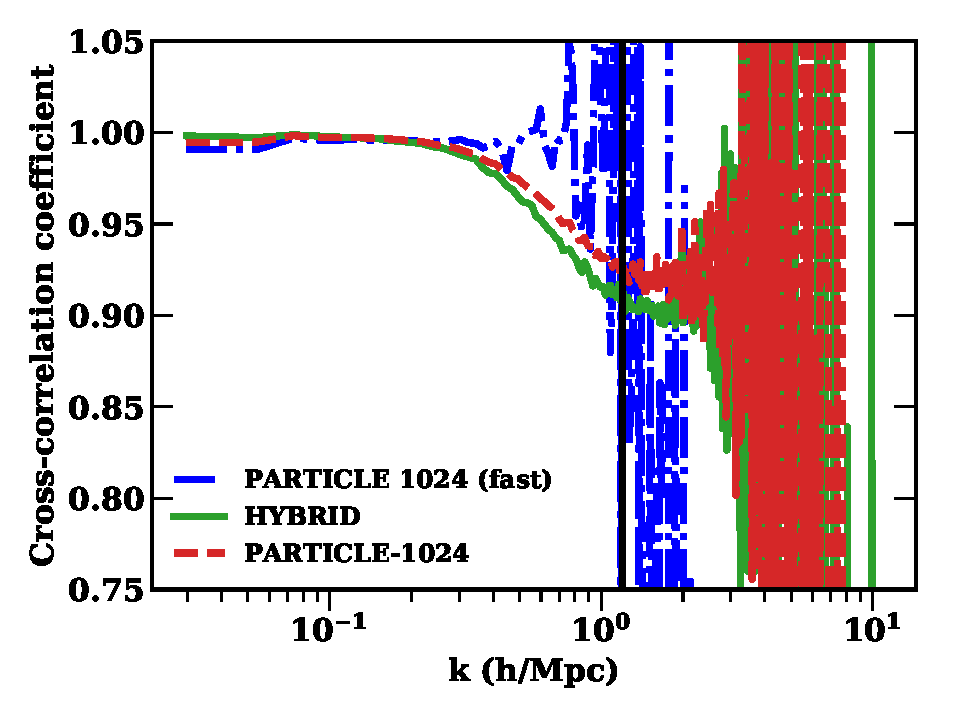
\includegraphics[width=0.45\textwidth]{nuplots/corr_coeff-1.pdf}
  \caption{The cross-correlation coefficient between neutrinos and dark matter using the particle and hybrid simulation methods.
  Shot noise has been subtracted from the neutrino power spectrum. For the hybrid simulation, only the correlation between the
  cold dark matter and slow neutrino particles is shown.
  The cross-correlation is unity for scales where the neutrino power is not dominated by shot noise (vertical dotted line),
  and $\sim 0.9$ for all scales larger than the mean interparticle spacing of the simulation. This justifies the
  approximation that neutrinos and CDM are completely correlated used in the linear response method.
  }
  \label{fig:cross-corr}
\end{figure}

\subsection{Hybrid method}
\label{sec:hybrid}

\begin{figure}
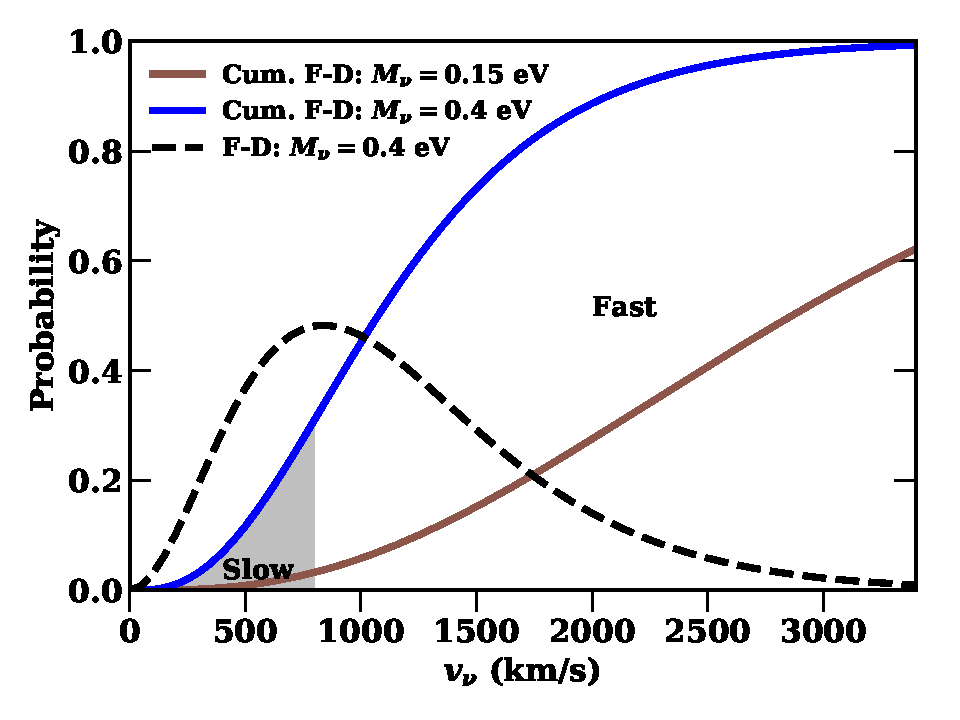
\includegraphics[width=0.45\textwidth]{nuplots/fermidirac.pdf}
  \caption{The integrated Fermi-Dirac distribution, showing the cumulative probability for neutrinos to have an unperturbed velocity less than $v_\nu$ at $z=0$ for total neutrino mass $M_\nu = 0.4$ eV.
  The grey shaded region shows the neutrino density followed by particles in our hybrid method.
  }
  \label{fig:fddistribution}
\end{figure}

In AHB13, the linear-response approximation was used for the \emph{entire} phase-space of neutrinos.
Yet, as discussed above, this approximation should eventually break down below some critical velocity, as neutrinos start to behave more similarly to the CDM. In fact, the velocity of neutrinos follows a Fermi-Dirac distribution, meaning that some fraction of the neutrinos will initially have near-zero velocities and be poorly described by the linear response approximation. Indeed, AHB13 showed that the linear response neutrino simulation method did not fully reproduce the neutrino power spectrum at late times and on small scales.
Even if slow neutrinos make up a small fraction of the total matter density, they can still dominate the total power spectrum because the clustering of the faster neutrinos is heavily suppressed.

To remedy this issue, we split neutrinos into a ``slow" and a ``fast" component. The split is defined in terms of the \emph{unperturbed} velocities: neutrinos whose initial velocity is less than a critical velocity $v_{\rm crit}$ are called slow, and the rest are called fast. Because at linear order velocity shells do not mix, neutrinos which are initially labelled as fast or slow remain within these categories throughout their evolution. As a consequence, both the slow and fast components independently satisfy the collisionless Boltzmann equation, which we are free to solve with different techniques. We use the linear-response technique for the fast component, whose over-densities remain small. We focus the computationally expensive $N$-body technique on the small fraction of slow neutrinos, for which it is really needed. The pure $N$-body method is recovered for $v_{\rm crit} \rightarrow \infty$, and the pure linear-response method of AHB13 is obtained in the limit $v_{\rm crit} \rightarrow 0$. Figure~\ref{fig:fddistribution} shows the Fermi-Dirac distribution, with the shaded area under the curve indicating the slow neutrino component.

In principle, the optimal critical velocity $v_{\rm crit}$ increases with time, as neutrinos redshift and gravitational potentials deepen. For example, while the CDM potential is linear, the desired critical velocity is zero. These early times are also exactly those where the neutrino thermal velocity and thus the impact of neutrino particle shot noise is largest. For this reason we follow all neutrinos using the linear response method until redshift $z_{\nu}$, when a significant fraction of the ``slow'' neutrinos cluster non-linearly. Our hybrid method thus avoids most of the effects of neutrino particle shot noise, and has two free parameters, $v_{\rm crit}$ and $z_{\nu}$.

\subsubsection{Choice of neutrino splitting parameters}
\label{sec:parameters}

\begin{figure}
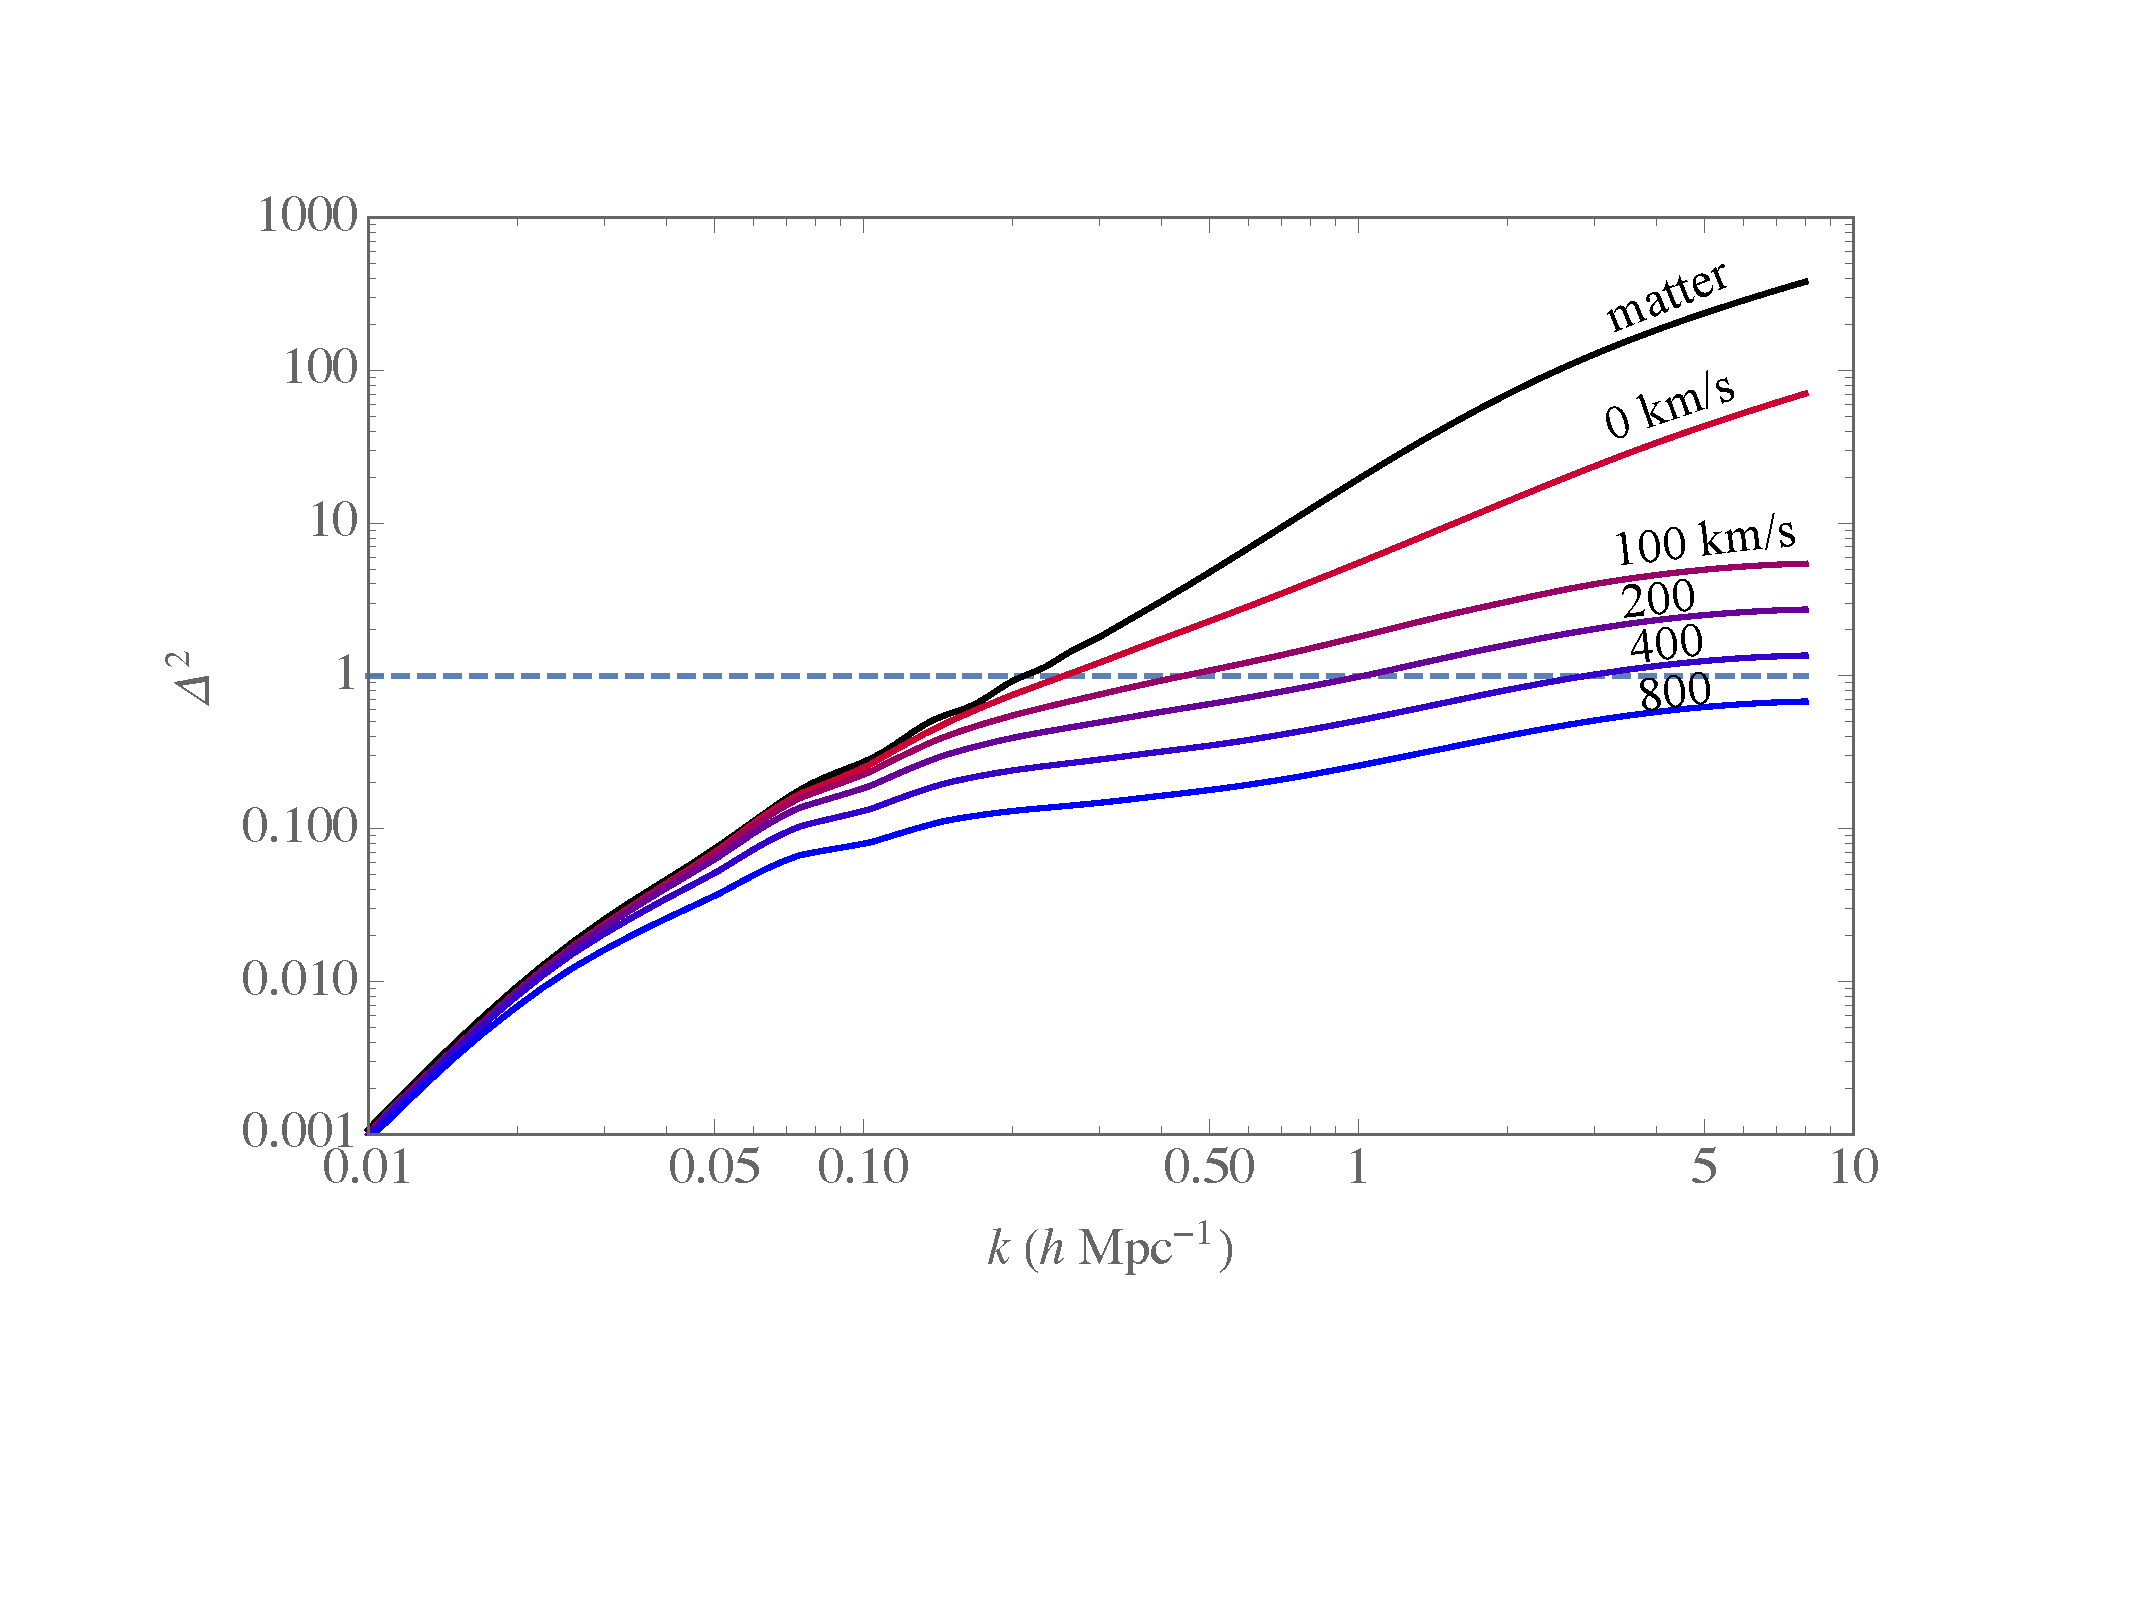
\includegraphics[width=0.45\textwidth]{nuplots/lin_resp_halofit.pdf}
\caption{The expected over-density of linear response neutrinos, demonstrating the critical velocity at which they are expected to become non-linear at $z=0$. \spb{Change velocities used to 0, 100, 400, 800, 1000, make labels bigger, shrink range, add redshift.} The expected neutrino power spectrum using our linear response approximation for a variety of different neutrino velocity shells. The matter power spectrum is computed using {\small HALOFIT}. Non-linear effects are expected for neutrino velocities where $\Delta^2 \gtrsim 1$.
  }
\label{fig:halofitvshell}
\end{figure}

\begin{figure}
  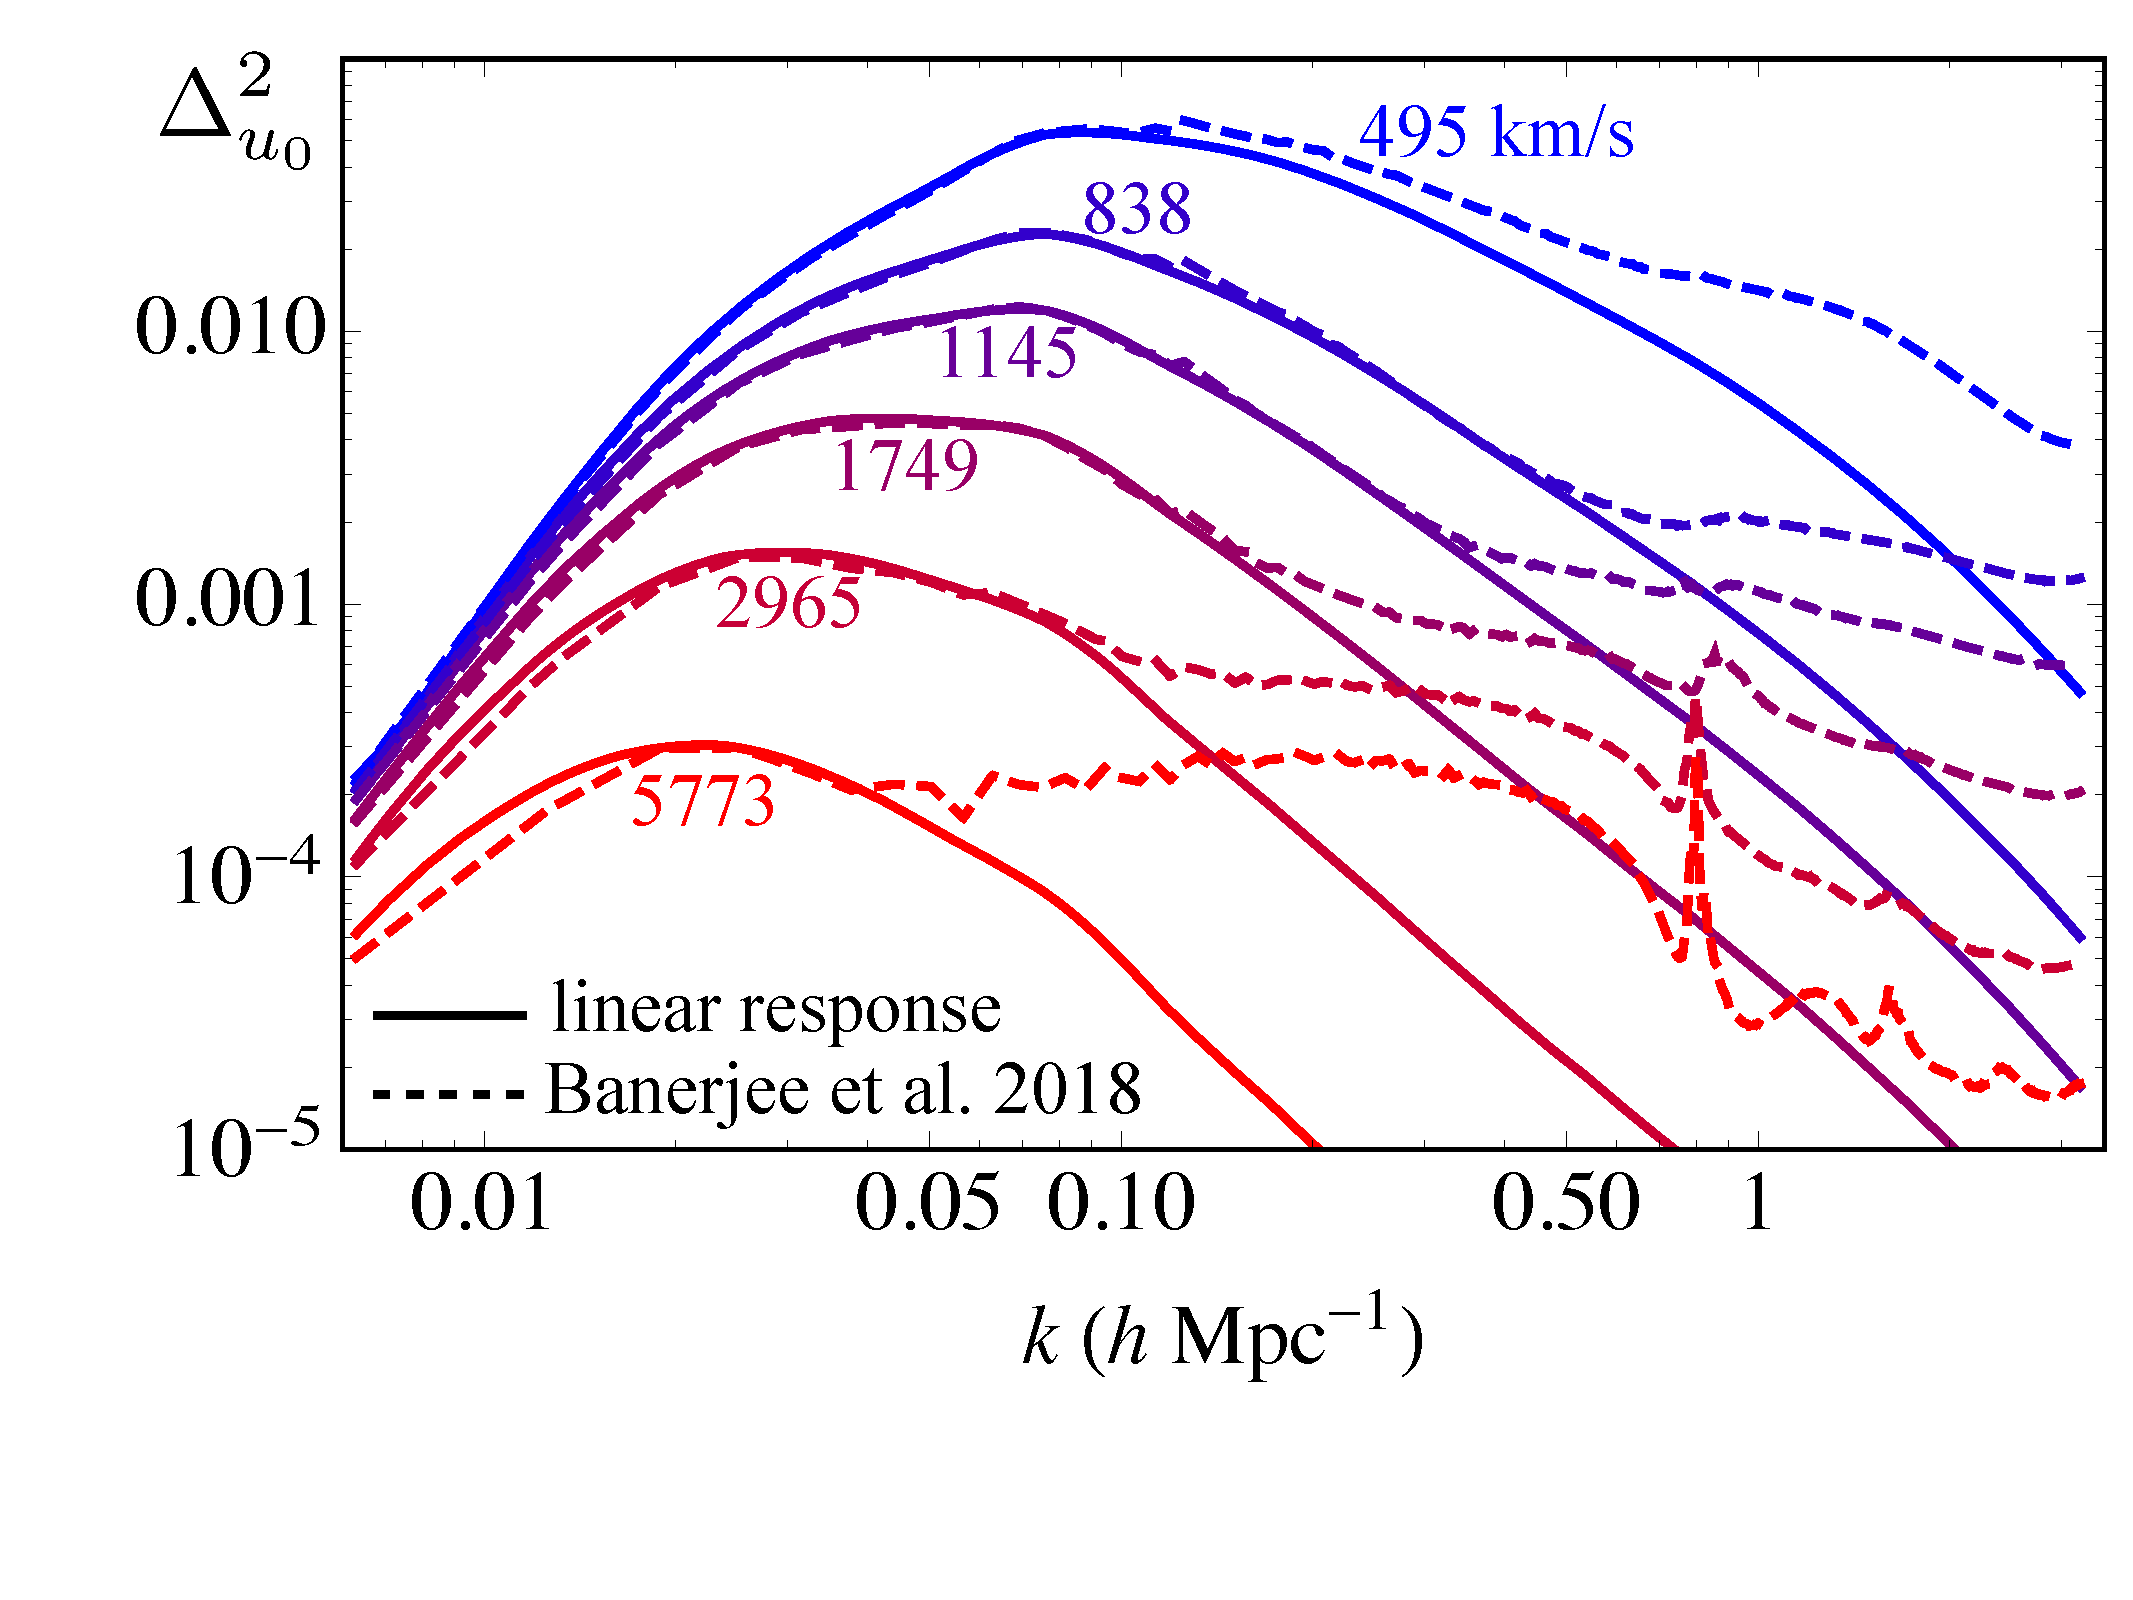
\includegraphics[width=0.45\textwidth]{nuplots/banerjee_lin_resp.pdf}
  \caption{
  The neutrino power spectrum in different velocity shells compared to the neutrino velocity shell simulations of \protect\cite{Banerjee_2018}. Excepting residual shot noise in their method, the linear response approximation provides accurate predictions for $v > 800$ km/s, as expected. \spb{I would like to include both plots: this one shows us that the particles and analytics match up to 800 km/s. The other shows us that we would expect them to match, because we are in a regime where perturbation theory works.}
  }
  \label{fig:simvshell}
\end{figure}

In this Section, we derive expectations for desired neutrino critical velocity and critical redshift.
We expect the linear response approximation to be accurate for a given neutrino velocity shell as long
as we are in a regime where the neutrino over-density in that shell remains less than unity, and thus described by perturbation theory. Figure~\ref{fig:halofitvshell} shows the expected neutrino power spectrum in a variety of velocity shells. Note that changing the neutrino mass alters the amount of neutrinos in each velocity shell, but does not alter the shell's evolution.

We used {\small HALOFIT} \cite{Smith_2003} to obtain approximate matter power spectra until $z=0$. These power spectra were used as sources in a linear response calculation for the shown power spectra, which assume a particle with a thermal velocity distribution given by a delta function. \spb{Yacine: is this what you did?} We then computed the expected dimensionless power spectrum for each velocity shell. We see that at $z=0$ the over-density is unity in a unperturbed velocity shell of $700 - 800$ km/s. Initially slower neutrinos will have over-densities significantly altered by non-linear graviational clustering, and so would not follow the expected linear response power spectra in Figure~\ref{fig:halofitvshell}.

Figure~\ref{fig:simvshell} validates our expectation using the neutrino velocity shell simulations of \cite{Banerjee_2018}. In these simulations, neutrinos are initialised in a variety of velocity bins, each of which we can compare to the expectation of our linear response approximation. We see that, as expected from Figure~\ref{fig:halofitvshell}, and excluding particle shot noise in the higher velocity shells, our linear response approximation is a good match for all shells with $v_\mathrm{crit} \geq 838$ km/s. To be conservative, we
thus use a default neutrino critical velocity of $850$ km/s. We expect all neutrinos initially faster than this value to be accurately followed to $z=0$. For the critical neutrino redshift, we performed a similar computation to Figure~\ref{fig:halofitvshell} at $z=1$, finding that $\Delta^2 > 1$ for $v_\mathrm{crit} = 100$, corresponding to $0.14\%$ of the neutrinos for $M_\nu  = 0.4$ eV. We thus conservatively set $z_\nu = 1$, although we caution that simulations which use a larger neutrino mass might require $z_\nu > 1$.

% We may get a simple estimate of the relevant $v_{\rm crit}$ from AHB13's analysis of the condition for neutrinos to escape a time-dependent potential: rewriting their equation (16), we find that the minimal velocity required to escape capture by a halo with characteristic extent $r_0$, potential $\phi_0$, varying on a timescale $\Delta t_\phi$, is
% \barr
% v \gtrsim 500 ~\textrm{km/s} ~ \left(\frac1{H_0 \Delta t_\phi} ~ \frac{r_0}{0.5~ h^{-1} \textrm{Mpc}}~ \frac{\sqrt{|\phi_0|}}{3000~ \textrm{km/s}} \right)^{1/2}.
% \earr
% We therefore expect that a critical velocity of several hundred km/s should be used. Our fiducial choice in this work is $v_{\rm crit} = 750$ km/s, which we discuss more in Section \ref{sec:results}.

% For reference, for a neutrino mass sum $M_\nu = 0.4$ eV, 28\% of neutrinos have velocities below 750 km/s.

%
%By default we consider the ``slow-moving '' tail of the Fermi-Dirac distribution to be all neutrino density with an unperturbed velocity less than $750$ (comoving) km/s. We found by experiment that this value was the smallest that led to good agreement
%with the particle neutrino method. The effects of other cutoff velocities are discussed in Section~\ref{sec:results}.
%The critical redshift at which particle neutrinos switched on was set at $z=1$, for similar reasons.

\subsubsection{Implementation of the split ``slow'' neutrinos}

We could in principle generate slow neutrino particles at $z_\nu$, the cutoff redshift after which some neutrinos are not followed accurately with the linear response approximation. We would then use the linear-response approximation to compute the initial neutrino overdensities and bulk velocities. Doing so accurately would require computing neutrino perturbations as a function of their thermal velocity. We would use Eq.~\eqref{eq:delta-phi} and its time derivative for $f_0(u)$ given by narrow distributions around velocity bins $u_i$\footnote{This would be equivalent to the multi-fluid method of \citealt{Dupuy_14}}.

Instead, we chose to generate slow neutrino particles at the initial simulation redshift $z_i = 99$, and follow them as tracer particles until $z_\nu$. Their trajectories are thus computed using the N-body technique in the total matter potential, comprising CDM and linear-response neutrinos. However, they themselves do not gravitate and affect the trajectories of other particles until after $z_\nu$\footnote{Note that the hybrid method of \cite{Brandbyge_2010} creates neutrino particles dynamically during the simulation, rather than initially treating them as tracers.}. The increased particle load still imposes some numerical overhead over the pure linear-response method, but allows for accurate ``initial" conditions for slow-neutrino particles at $z_\nu$.

In our tests, before $z_\nu$, the hybrid particle simulations were about $35\%$ slower than the linear response simulations, while a pure particle simulation was about $150\%$ slower with the same particle load.
The numerical overhead is thus substantially reduced for the hybrid method over pure particle neutrino simulations. This is because the neutrino particles have a slower average velocity in the hybrid method and thus longer timesteps.

Simulating slow neutrino trajectories from $z_i = 99$ also allows us to start from completely homogeneous initial conditions, i.e. neglect any initial overdensities and bulk velocities. We verified explicitly that our results at all redshifts were unchanged for a simulation where our slow-moving neutrinos had an initial clustering matching the transfer function of the CDM, a conservative over-estimate of their true initial clustering.

For ease of comparison with particle simulations, the simulations presented in this paper assume that all three neutrino species are degenerate. Neutrino masses small enough that the neutrino hierarchy is important, $M_\nu < 0.15$~eV, have $\lesssim 3$\% of neutrino initial velocities $< 800$ km/s. AHB13 showed that the linear response method is able to accurately model the neutrino power spectrum at these masses. Future hybrid simulations including a neutrino hierarchy would generate particles only for the most massive neutrino species, as for particle simulations. \spb{What I had before was perhaps overly negative...}


\subsubsection{Implementation of the split ``fast'' neutrinos}

After the slow neutrinos have begun to gravitate, the linear response approximation must be modified to include only the ``fast'' neutrinos, that is, the portion of the neutrino phase space with unperturbed velocities higher than the cutoff velocity. Here we describe how the equation of the linear response approximation described in Section~\ref{sec:analytic} are modified to describe this case.

The unperturbed phase-space density of the fast neutrinos is
\begin{equation}
f_0(u) \propto \Theta(u - v_{\rm crit}) \left(\rme^{m_\nu u/T_\nu} + 1 \right)^{-1},
\end{equation}

where $\Theta$ is the Heaviside function (or an infinitesimally smoothed version of it, so that $f_0$ is differentiable), $m_\nu$ is the mass of a single neutrino or antineutrino, and $T_\nu \approx 1.68 \times 10^{-4}$ eV is the temperature of the cosmic neutrino background. The normalization is again such that $\int d^3 u f_0(u) = 1$. The kernel in Eq.~\eqref{eq:delta-phi} is therefore given by
\barr
\mathcal{I}(\kappa) = \frac{\int_{q_c}^{\infty} dq~ j_0\left(\kappa \frac{T_\nu}{m_\nu}q\right)~ q^2 /(\rme^q + 1) }{\int_{q_c}^{\infty} dq ~q^2/(\rme^q + 1)}, \ \ \ q_c \equiv \frac{m_\nu v_{\rm crit}}{T_\nu}.
\earr
We use the following asymptotic expansion for the integral:
\begin{align}
 \int^\infty_{q_\mathrm{c}} \frac{j_0(qX)}{e^q + 1} q^2 dq &= - \sum^{\infty}_{n=1} (-1)^n \frac{\rme^{-n q_\mathrm{c}}}{(n^2+X^2)^2} I_n(q_\mathrm{c},X),\\
 I_n(q_\mathrm{c},X) &= \left(n^2 + n^3 q_\mathrm{c} + n q_\mathrm{c} X^2 - X^2\right) \frac{\sin(q_\mathrm{c} X)}{X} \nonumber \\
 &+ \left(2n + n^2 q_\mathrm{c} + q_\mathrm{c} X^2\right) \cos(q_\mathrm{c} X),
\end{align}
which we have confirmed, using Mathematica, to have an absolute error of $< 10^{-4}$ for $n_\mathrm{max} = 20$.

\subsection{Simulations}
\label{sec:simulations}

%TABLE OF SIMULATIONS.
\begin{table}
\begin{center}
\begin{tabular}{|l|c|c|c|c|l|}
\hline
% Name & $M_\nu$ (eV) & Method & Box (Mpc/h) & $N_\mathrm{part}^{1/3}$ & Notes \\
% \hline
%     &       0             &    -          & 512         & 512       &       \\
%     &       0             &    -          & 300         & 512       &       \\
%     &     0.4             &   Analytic    & 300         & 512       &       \\
%     &     0.4             &   Particle    & 300         & 512       &       \\
%     &     0.4             &   Hybrid      & 300         & 512       &  $256^3$ nu particles    \\
%     &     0.4             &   Hybrid      & 300         & 512       &  $256^3$ nu particles    \\
%     &     0.4             &   Hybrid      & 300         & 512       &  $256^3$ nu particles    \\
%     &     0.4             &   Hybrid      & 300         & 512       &  $256^3$ nu particles    \\
%     &     0.4             &   Hybrid      & 300         & 512       &  $256^3$ nu particles    \\
    Name & $M_\nu$ (eV) & Method & $N_\nu^{1/3}$ & $v_\mathrm{crit}$ & Notes \\
\hline
CDM    &       0             &    -          & 0         & - &    \\
MINNU    &     0.06            &   Lin. Resp.    & 0         & - &  NH  \\
LINRESP    &     0.4             &   Lin. Resp.    & 0         & - &    \\
PARTICLE    &     0.4             &   Particle    & 512       & - &    \\
2xPARTICLE    &     0.4             &   Particle    & 1024 & - &    \\
%     &     0.4             &   Hybrid      & 256     &   &    \\
HYBRID    &     0.4             &   Hybrid      & 512       & 850 & \\
HYBSING    &     0.4             &   Hybrid      & 256       & 850 & \\
NUTIME    &     0.4             &   Hybrid      & 512       & 850 & $z_\nu = 4$  \\
VCRITLO    &     0.4             &   Hybrid      & 512       & 750 & \\
VCRIT    &     0.4             &   Hybrid      & 512       & 1000 & \\
HYBALL    &     0.4             &   Hybrid      & 512       & 5000 & $z_\nu = 1$ \\
%    &     0.4             &   Hybrid      & 512       & 500 &    \\
% Note HYBALL and NUTIME are swapped compared to their directory names
\hline
\end{tabular}
\end{center}
\caption{Table of simulations performed. All simulations have a box of $300$ Mpc/h
and $512^3$ CDM particles. NH denotes a normal hierarchy for the neutrino masses.
For $M_\nu = 0.4$ eV, the fraction of neutrinos slower than critical velocities of $750$, $850$, $1000$, $5000$ km/s is $0.276$, $0.346$, $0.451$ and $1$ respectively. \yah{are names necessary, or can we go with S1, S2, etc...?} \spb{I always find names easier to follow...}}
\label{tab:simulations}
\end{table}

% Mnu = 0  (300)

% Mnu = 0.4: analytic, particle, hybrid. (300)
%
% Checks (all Mnu=0.4, hybrid, (300)):
% Varying vcrit from 500 to 300
% Varying NuPartTime from 0.333 to 0.5
% Number of hybrid particles from 256 to 512.
% Mnu = 0.06: analytic (300, 512)

Our simulations were run with MP-Gadget\footnote{\url{https://github.com/rainwoodman/MP-Gadget/}} and are detailed in Table \ref{tab:simulations}. We used a box size of $300$ comoving Mpc/$h$ with $512^3$ CDM particles.
The CDM particles were initialised using a linear transfer function generated at $z=99$ with massive neutrinos using CAMB \citep{CAMB_neutrinos}. Each simulation has the same initial phases, ensuring the same distribution of late-time halos. We performed simulations with massless neutrinos, and a linear response simulation with the minimal neutrino mass allowed by oscillation experiments, $M_\nu = 0.06$ eV (and a normal neutrino hierarchy). All other simulations have a total neutrino mass of $0.4$~eV, and assume a degenerate neutrino hierarchy. This relatively high neutrino mass $0.4$~eV was chosen to make the different predictions of the linear response and hybrid methods for the neutrino power spectrum easier to visualize.

We performed three simulations using these parameters and identical except for the neutrino simulation method. These simulations used the linear response method, particle neutrinos and our new hybrid implementation. We then performed a number of simulations designed to test the sensitivity of our hybrid method to numerical parameters. Our default hybrid neutrino simulation had neutrinos with an unperturbed velocity of $850$ (comoving) km/s followed by $512$ neutrino particles (matching the CDM) and a neutrino switch-on time of $z_\nu = 1$. Our modified simulations considered the effects of a neutrino switch-on time of $z_\nu = 4$, of only $256^3$ neutrino particles, and critical unperturbed velocities of $1000$ and $5000$ km/s. The simulation with a critical velocity of $5000$ km/s includes all the neutrino power in particles after the neutrino switch-on time and is useful as a comparison to the pure particle method. We finally performed a simulation with a critical velocity of $500$ km/s, which differed from the simulation with a critical neutrino velocity of $850$ (comoving) km/s by up to $20\%$.

\section{Results}
\label{sec:results}

\begin{figure*}
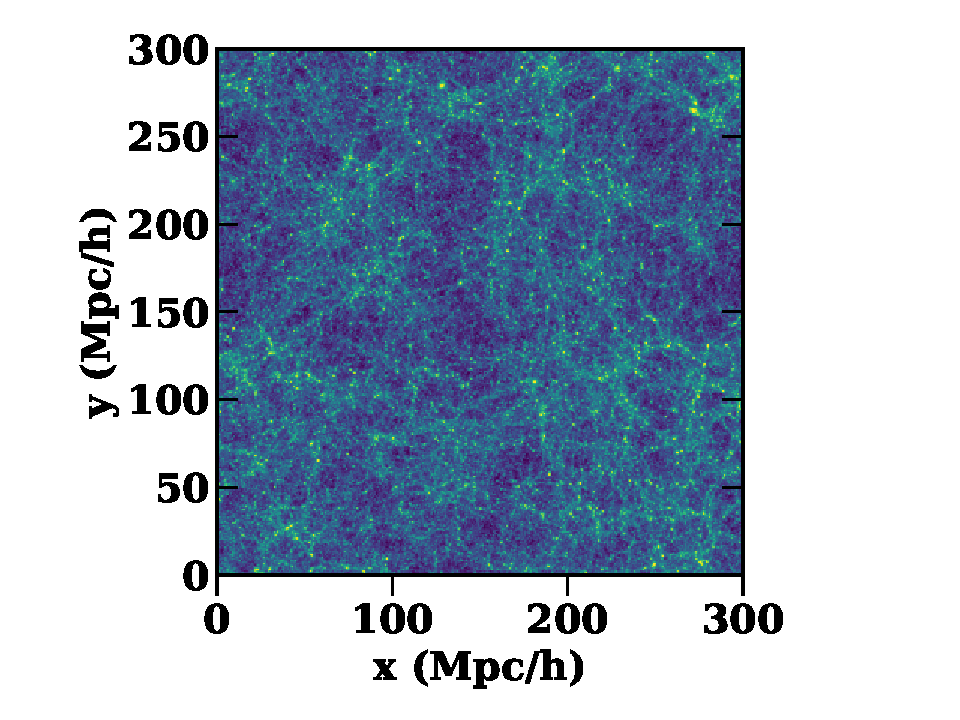
\includegraphics[trim={1.cm 0 1.5cm 0},clip,width=0.31\textwidth]{nuplots/dens-plt-b300p512nu0_4hybt1.pdf}
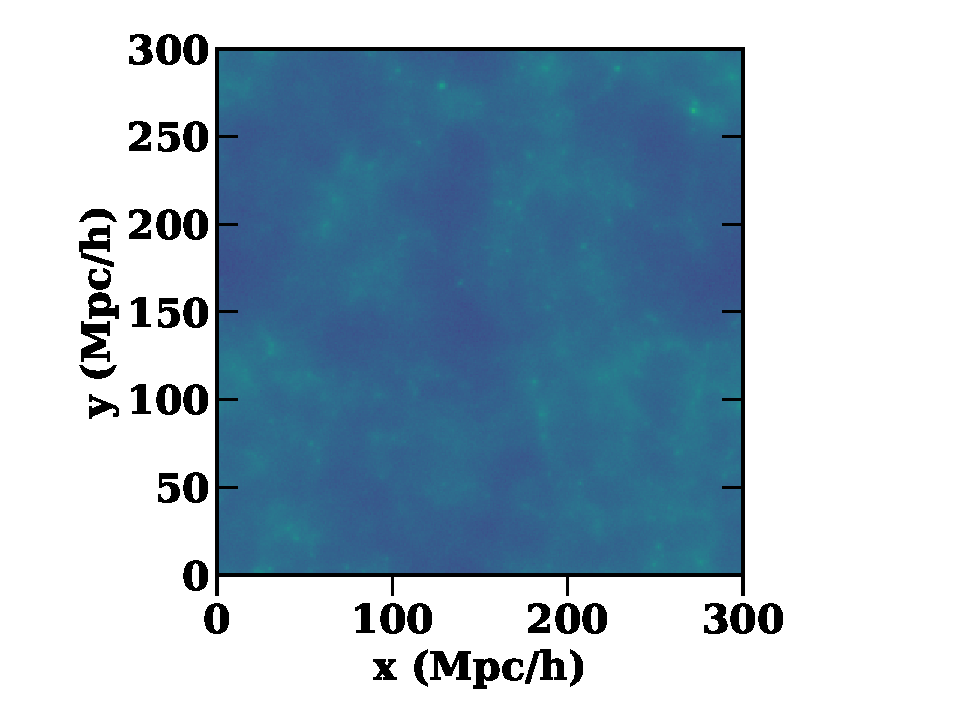
\includegraphics[trim={1cm 0 1.5cm 0},clip, width=0.31\textwidth]{nuplots/dens-plt-b300p512nu0_4hybt2.pdf}
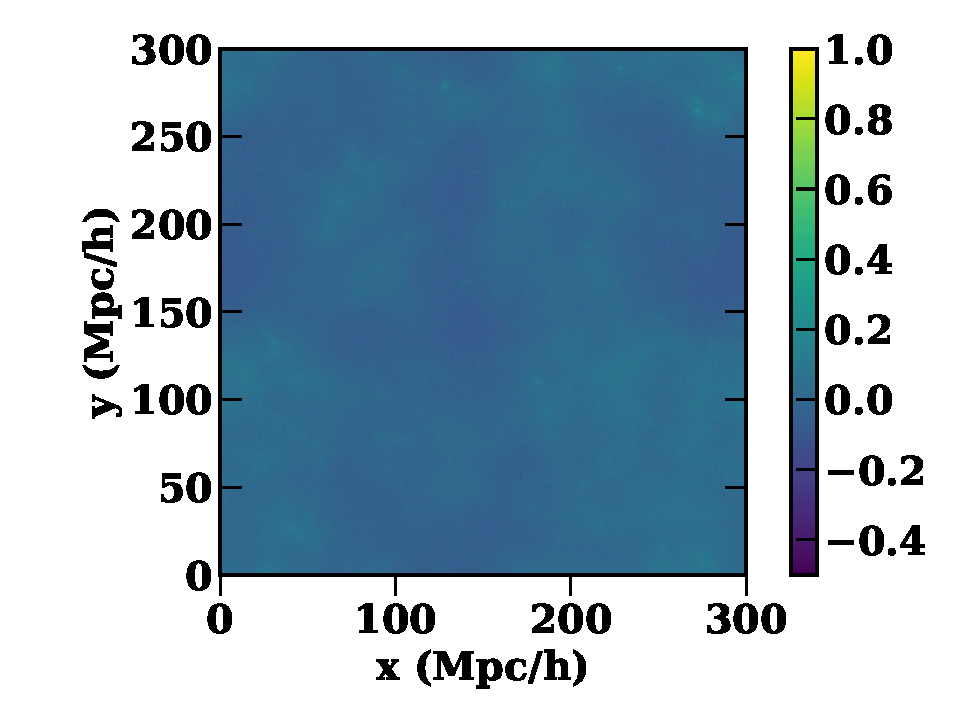
\includegraphics[trim={1.5cm 0 0.5cm 0},clip, width=0.322\textwidth]{nuplots/dens-plt-b300p512nu0_4pt2.pdf}
  \caption{Projected density plots at $z=0$. \emph{Left}: CDM. \emph{Middle}: Neutrino particles from the hybrid simulation, with unperturbed velocity $<850$ (comoving) km/s. \emph{Right}: Neutrino particles from the pure particle simulation, i.e. including neutrinos from all unperturbed velocities. Colours show $\log (1+ \delta)$ in dimensionless units, where $\delta$ is the projected over-density.
  %No correction has been made for shot noise \yah{what would such a correction even mean for this kind of plot??}.
  The clustering of the hybrid particles is intermediate between that of the cold dark matter and the particle neutrinos. Structures have the same positions in all three panels. \yah{It would be super nice to show the density of linear-response neutrinos...} \spb{Not sure how to do that}}
  \label{fig:density_plot}
\end{figure*}

\begin{figure*}
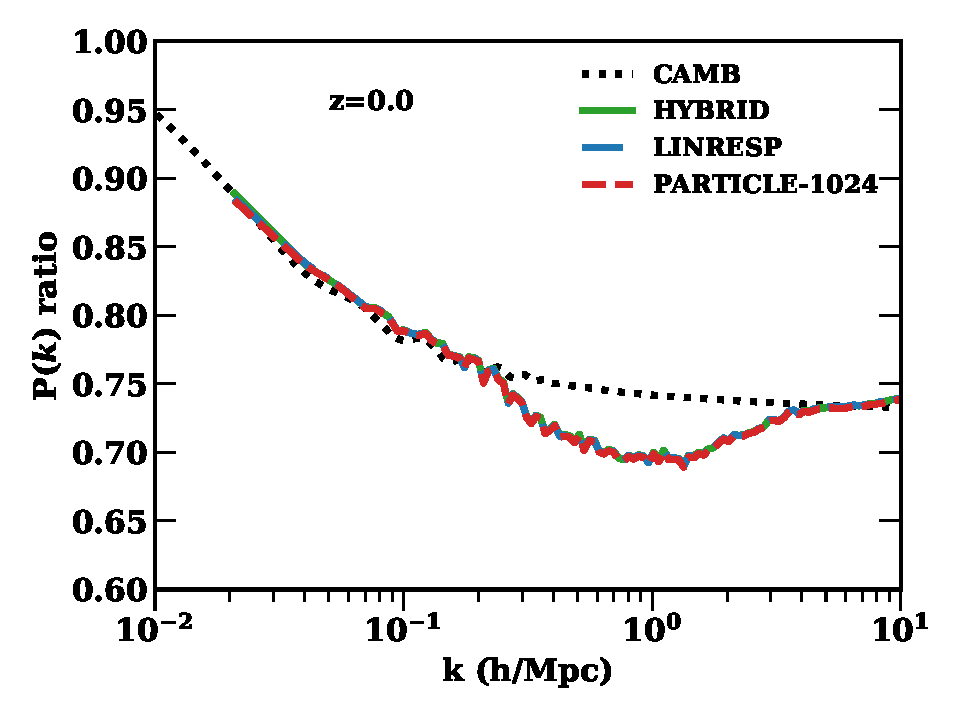
\includegraphics[width=0.45\textwidth]{nuplots/pks_rel-10.pdf}
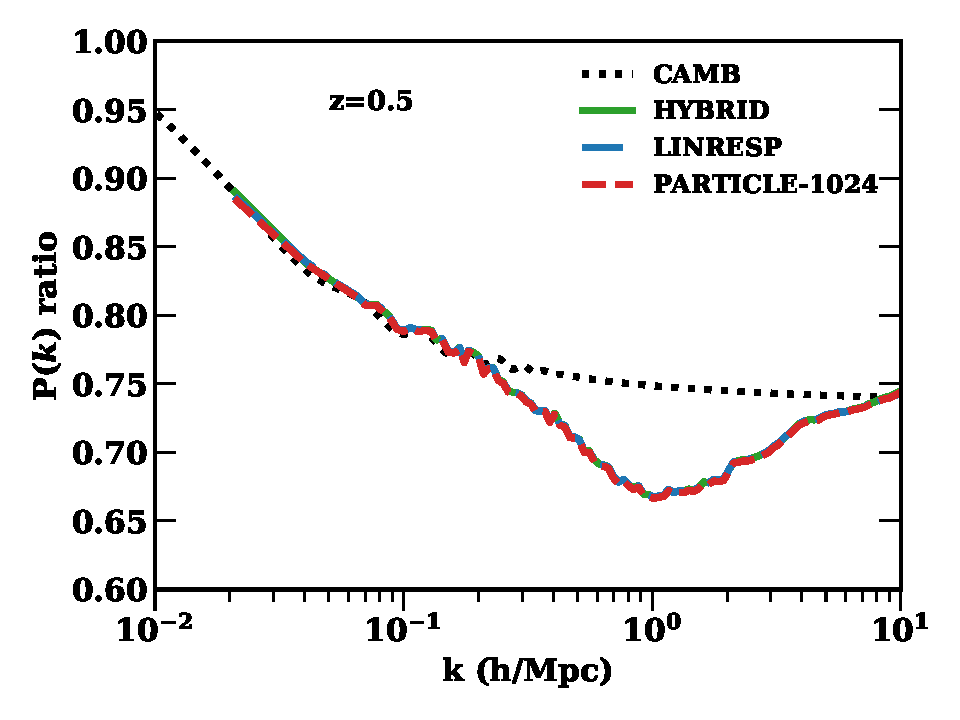
\includegraphics[width=0.45\textwidth]{nuplots/pks_rel-0_66670.pdf}
  \caption{Ratio of matter power spectrum with massive neutrinos ($M_\nu = 0.4$ eV) to matter power spectrum with massless neutrinos. Figure shows hybrid (HYBRID), linear response (LINRESP), and particle (2xPARTICLE) methods at (Left) $z=0$ and (Right) $z=0.5$. All three simulation methods agree with $\sim 0.1$\%, in agreement with AHB13. Achieving convergence for the particle neutrino method required a large number of neutrino particles, and thus almost an order of magnitude more CPU time, as discussed in Section~\ref{sec:matterpower}.
  }
  \label{fig:matter_power}
\end{figure*}

\begin{figure}
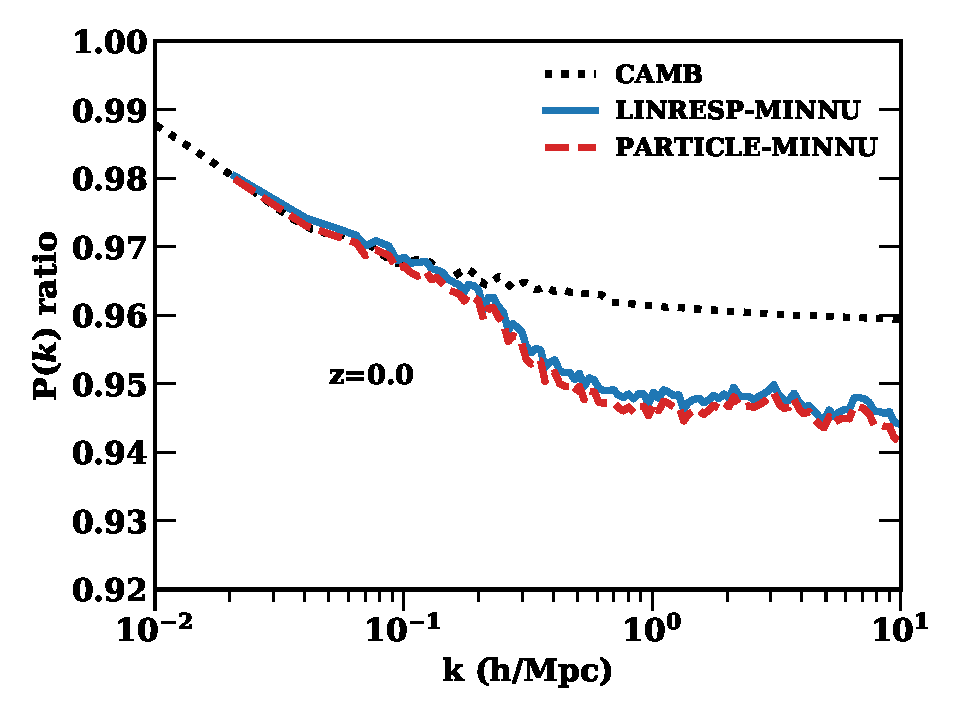
\includegraphics[width=0.45\textwidth]{nuplots/pks_lowmass-10.pdf}
\caption{Ratio of the matter power spectrum with the minimal neutrino mass ($M_\nu = 0.06$ eV) to the matter power spectrum with massless neutrinos at $z=0$. The linear response method (MINNU) and particle method (MINNU-PART) are shown. At these low masses, the particle method is affected by shot noise.
}
\label{fig:minimal_mass}
\end{figure}

\begin{figure*}
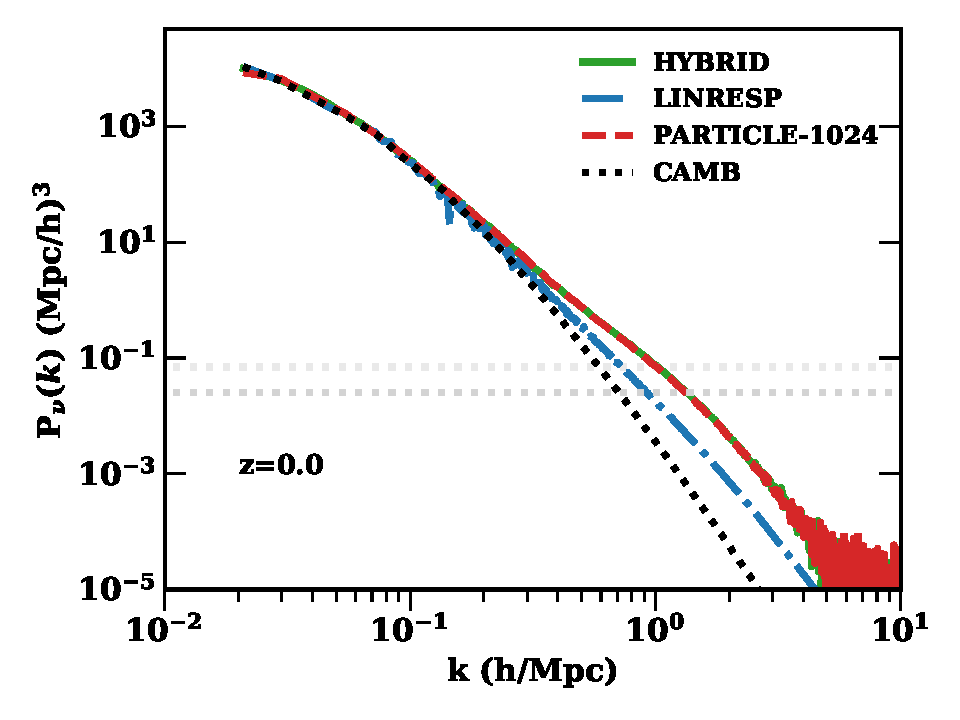
\includegraphics[width=0.45\textwidth]{nuplots/pks-nu-1.pdf}
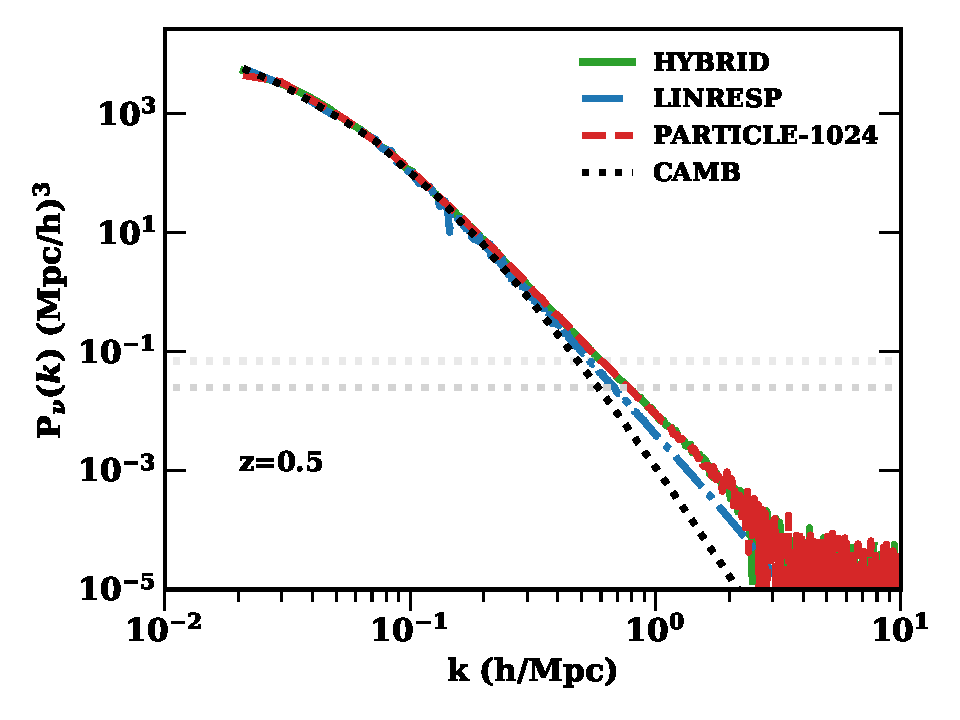
\includegraphics[width=0.45\textwidth]{nuplots/pks-nu-0_6667.pdf}
  \caption{The neutrino power spectrum with massive neutrinos ($M_\nu = 0.4$ eV) for simulations using linear response (LINRESP) hybrid (HYBRID) and particle (PARTICLE) methods. (Left) At $z=0$. (Right) At $z=0.5$. We have subtracted shot noise from the particle and hybrid simulations. The heavier dashed grey curve shows the level of shot noise subtracted from the particle simulation, while the lighter dashed grey curve shows the level subtracted from the hybrid simulation. We show the linear theory neutrino power spectrum from CAMB for comparison. There is good agreement between the hybrid and particle simulation methods.}
  \label{fig:neutrino_power}
\end{figure*}

\begin{figure}
\includegraphics[width=0.45\textwidth]{nuplots/pks_nu_rel-1.pdf}
  \caption{The ratio of the neutrino power spectrum for simulations using linear response (LINRESP) and particle (PARTICLE) methods to the hybrid simulation (HYBRID) at $z=0$. Also shown is the linear theory neutrino power spectrum from CAMB. We have subtracted shot noise from the particle and hybrid simulations.}
  \label{fig:rel_neutrino_power}
\end{figure}

\begin{figure}
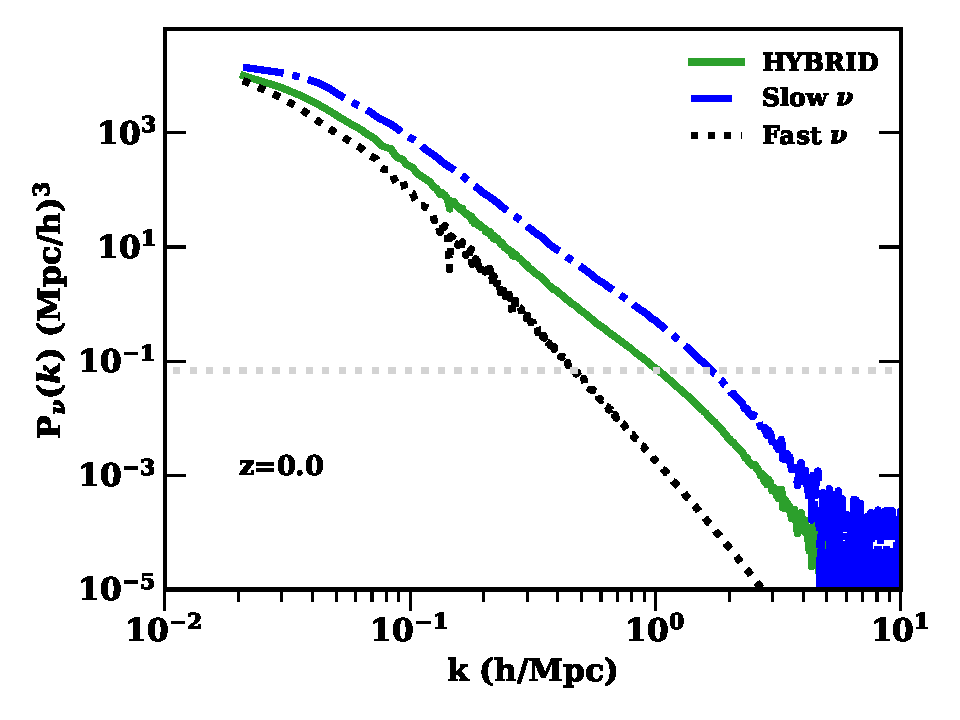
\includegraphics[width=0.45\textwidth]{nuplots/pks-nu-split-1.pdf}
  \caption{The neutrino power spectrum for the hybrid simulation (HYBRID) at $z=0$, split into fast (analytic) and slow (particle) neutrino components. Shot noise has been subtracted at the level shown by the grey line.}
  \label{fig:neutrino_power_split}
\end{figure}

Figure \ref{fig:density_plot} shows projected densities for the CDM and neutrino particles from the HYBRID and PARTICLE simulations.\footnote{Projected density plots made using Nbodykit.}, in order to give a visual impression of the clustering of the neutrinos and dark matter. The structure of filaments, halos and voids is identical in all three plots, further reinforcing the conclusion of Figure \ref{fig:cross-corr} that the phases of the neutrinos and CDM are highly correlated. The neutrino particles in the hybrid simulation cluster more than in the purely particle simulation, but in both cases less than the CDM. This matches the expected behaviour given their lower initial thermal velocities.

\subsection{Matter Power}
\label{sec:matterpower}

Figure~\ref{fig:matter_power} shows the $z=0$ and $z=0.5$ matter power spectrum for all three neutrino simulation methods: particle, linear response and hybrid. These three simulations are identical except for the method used to follow neutrino perturbations. In particular, they all use the same cosmological background solution, which includes radiation and massive neutrinos. Figure~\ref{fig:matter_power} shows the ratio of the matter power spectrum in each simulation with massive neutrinos compared to the matter power spectrum from a pure-CDM massless neutrino simulation. We also show the linear theory evolution from CAMB. Validating our new hybrid method, the hybrid and linear response simulation methods produce matter power spectra which are indistinguishable by eye from the particle method, and in fact differ by around $0.1\%$. They also agree well with linear theory on linear scales, $k < 0.2$ $h$/Mpc.

The particle neutrino simulation contains $1024^3$ neutrino particles, $8\times$ the number of CDM particles. This high particle load increased the computational cost by a corresponding factor of $8$ (note that our simulation includes the short-range gravitational force for the neutrinos). A simulation with $512^3$ neutrino particles was not fully converged. We found that between $z=99$ and $z=49$ the simulation underestimated the growth of the matter power spectrum by approximately $1\%$, independently of scale. AHB13 avoided this discrepancy with linear theory by starting their simulations at a lower redshift ($z=49$), but this leads to inaccuracy in the CDM power spectrum \citep{Heitmann:2010}. A strength of our hybrid and linear response methods is that the particle neutrinos do not gravitate until late times, when the neutrino power spectrum is no longer shot noise dominated. To demonstrate this explicitly, we performed a hybrid simulation where all neutrinos are followed by the particle component (HYBALL in Table \ref{tab:simulations}, discussed in Section \ref{sec:check}). Thus this simulation is identical to the linear response simulation before the particle switch-on time of $z=1$ and identical to the particle simulation thereafter. Like the simulations shown in Figure \ref{fig:matter_power}, it produces a matter power spectrum in good agreement with CAMB.

Figure \ref{fig:minimal_mass} shows the results of simulations with $M_\nu = 0.06$~eV $z=0$. These low neutrino masses will become increasingly important as the upper limit on $M_\nu$ is reduced. We show linear response and particle simulations, but omit a hybrid simulation as for this neutrino mass $ < 4\%$ of the neutrinos have an initial velocity greater than $850$ km/s. The particle simulation neglects the contribution of the two light neutrino species, with masses $0.01$ and $10^-3$~eV respectively, as only one neutrino mass state can be followed in a particle simulation\footnote{The background evolution is however identical to the linear response simulation.}. The linear response simulation agrees with linear theory for $k < 0.2$ h/Mpc, further demonstrating that our simulations are able to reproduce the results of linear theory on large scales even for the lowest neutrino mass allowed by oscillation experiments.

There is a discrepancy between the particle simulation and the linear response simulation. We have verified that it is the particle neutrino simulation which is discrepant with linear theory. This discrepancy occurs because the particle neutrinos are strongly affected by shot-noise. Our particle simulation used $512^3$ particle neutrinos, matching the number of CDM particles. Ensuring that the neutrino power spectrum is not shot noise dominated at $z=99$ would require $2048^3$ particles for $M_\nu = 0.06$ eV, which is beyond our computational capabilities. The effect of shot noise causes the power particle and linear response power spectra to grow steadily more discrepant between $z=9$ and $z=1$, as the particle neutrinos continue to be shot noise dominated even at low redshift.

\subsection{Neutrino Power}
\label{sec:nupower}

Figure~\ref{fig:neutrino_power} shows the neutrino power spectrum at $z=0$ and $z=0.5$ for the same three simulations, demonstrating each of the neutrino simulation methods, as well as the linear theory power spectrum from CAMB. For the hybrid simulation we have computed the total neutrino power spectrum (assuming both neutrino components are completely correlated) as the weighted sum of the power spectrum of the fast and slow components $P^{1/2}_\nu = f_\mathrm{fast} P^{1/2}_\mathrm{fast} + f_\mathrm{slow} P^{1/2}_\mathrm{slow}$, where $f_\mathrm{fast} + f_\mathrm{slow} = 1$. Figure~\ref{fig:neutrino_power_split} shows the neutrino power spectra for each individual component, demonstrating that the slow neutrinos do indeed cluster substantially more.

Neutrino particle shot noise has been subtracted from both the particle and hybrid simulation. The neutrino power is recoverable even two orders of magnitude below the shot noise level, indicating that there is little structure formation arising purely from neutrino shot noise. The shot noise for the hybrid simulation is reduced by $0.27$, corresponding to the reduced fraction of matter density in particle neutrinos, and demonstrating an advantage of the hybrid approach. \yah{Is it really remarkable? This means that the power spectrum is essentially computed with two digit precision... } \spb{It surprised me, because I expected the neutrino shot noise to source numerical structure at some level.} Conceptually, the hybrid approach focuses expensive computational resources where it is really needed, on slow neutrinos which cluster non-linearly.

Both particle and hybrid methods show sharply increased neutrino power on small scales over the linear response method. At $z \geq 1$ all three methods are in good agreement, consistent with the results of AHB13. However, Figure~\ref{fig:neutrino_power} demonstrates that the hybrid neutrino simulation reproduces the neutrino power spectrum of the particle simulation on small scales at $z = 0$ and $z=0.5$. As Figure~\ref{fig:rel_neutrino_power} shows, the particle and hybrid simulations differ quantitatively by $10\%$ at $k=1$ $h$/Mpc, with the hybrid simulation producing more power. This difference is consistent with the expected effect of increased mass resolution in the hybrid simulation. The particle simulation also produces $5\%$ more power than the hybrid simulation for $k < 0.1$ $h$/Mpc (in moderately better agreement with CAMB). Figure \ref{fig:vcrit} shows this excess is not present in the HYBALL simulation, which is identical to the particle simulation for $z < 1$. This may indicate it is due to the dynamical effects of neutrino particle shot noise at early times. For $k < 0.1$ h/Mpc, the hybrid and linear response simulations also agree at the $1\%$ level, with the linear response simulation in marginally better agreement with CAMB, although the difference is small.

In summary, our new hybrid method agrees well with CAMB on linear scales, for both neutrino and matter power spectrum. It reproduces the non-linear matter growth function of both particle and linear response simulations, and the non-linear neutrino growth seen in the particle simulation, with somewhat higher resolution.

\subsection{Halo Mass Functions}
\label{sec:halomass}

\begin{figure}
  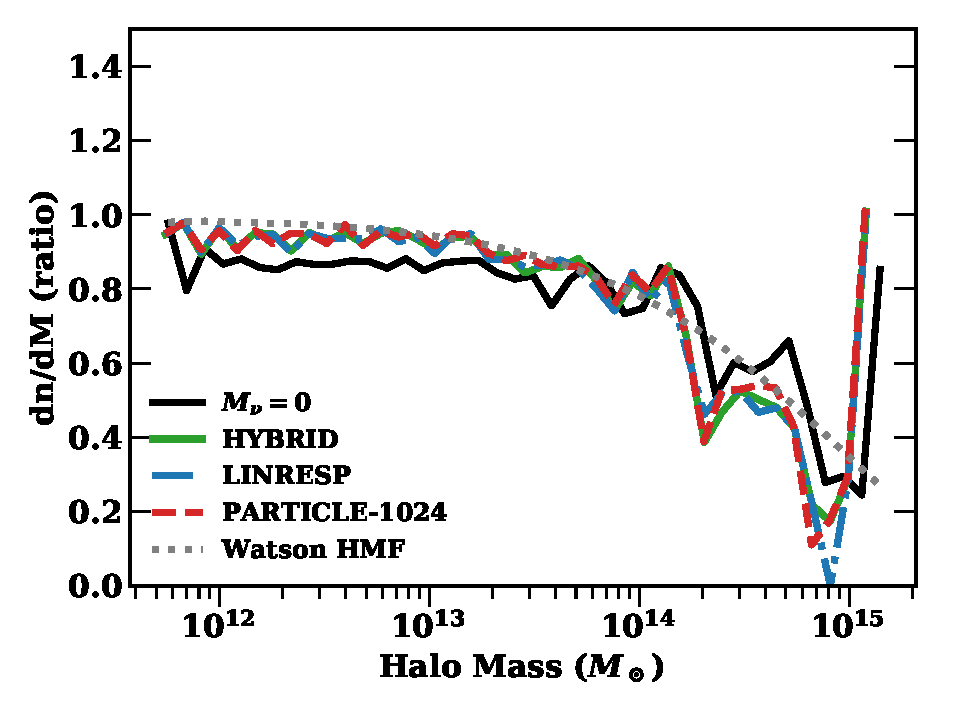
\includegraphics[width=0.45\textwidth]{nuplots/hmf-0_8333.pdf}
\caption{The halo mass functions at $z=0.2$ for our particle, linear response and hybrid simulations with $M_\nu = 0.4$ eV, as well as the mass function model from \protect\cite{Watson_2013} with parameters matching the massive neutrino model. We normalise by the mass function model with parameters corresponding to $M_\nu = 0$.}
  \label{fig:halomass}
\end{figure}

Figure~\ref{fig:halomass} shows the halo mass functions for our particle, linear response and hybrid simulations. The contribution from analytic (linear-response) neutrinos to the halo mass is approximated as zero. We show also a mass function model from \cite{Watson_2013}, with $\sigma_8 = 0.7372$, matching the linear power spectrum amplitude for the massive neutrino model. We also set $\Omega_M = \Omega_CDM + \Omega_b$ (ie, excluding the neutrino component), as recommended by \cite{FVN_2014}. All curves are normalised by a mass function model from \cite{Watson_2013} corresponding to our $M_\nu = 0$ cosmology, with $\sigma_8 = 0.8375$. We choose \cite{Watson_2013} because their calibration simulations use a friends-of-friends mass function with a linking length of $0.2$, as do our simulations. A model is used instead of a simulation to reduce scatter from Poisson noise, and $z=0.2$ is used instead of $z=0$ for the same reason. Our simulations agree reasonably well with the mass function model, although there is considerable scatter, perhaps indicating that our box size is insufficiently large. The simulated mass functions also agree well with each other. No systematic offset between simulation methods is visible, but we observe a $5\%$ scatter between individual mass bins. This may be due to chance inter-positions of neutrino particles between halos. The friends-of-friends algorithm would such particles as inter-halo links, even though they are not dynamically bound. We defer a more detailed analysis with more sophisticated halo finders and larger boxes to future work.

\subsection{Sensitivity to Model Parameters}
\label{sec:check}

\begin{figure*}
  \includegraphics[width=0.45\textwidth]{nuplots/pks-cknu-1.pdf}
  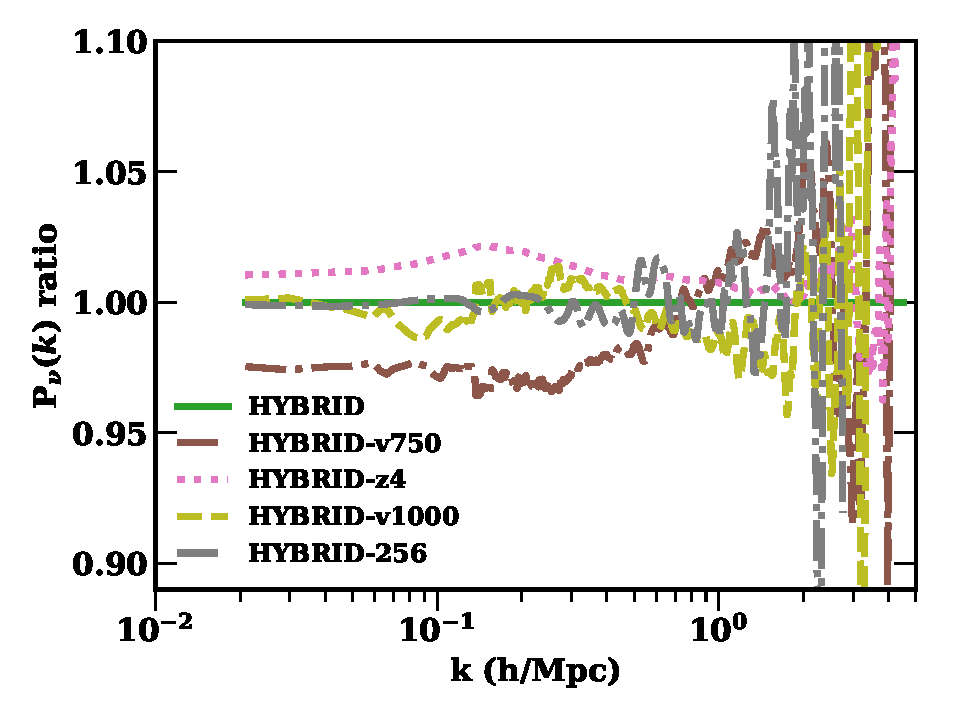
\includegraphics[width=0.45\textwidth]{nuplots/pks_nu_ckrel-1.pdf}
\caption{(Left) The effect of changing our hybrid model parameters on the neutrino power spectrum at $z=0$. We have varied the neutrino switch-on time, the critical neutrino velocity and the number of neutrino particles. We show the linear theory power spectrum from CAMB for comparison. We have subtracted shot noise at the level shown by the dashed grey curve. (Right) Ratio of neutrino power spectra to the results of the default hybrid simulation parameters (HYBRID). Data has been smoothed with at $15$-point Hanning filter to reduce numerical noise.}
  \label{fig:vcrit}
\end{figure*}

Figure~\ref{fig:neutrino_power} demonstrated that the hybrid neutrino method is capable of reproducing the neutrino power spectrum of a particle simulation, with substantially lower levels of shot noise. In this Section we show the sensitivity of our neutrino power spectrum measurement to various parameters of the hybrid model. In particular, we have varied the neutrino switch-on time, the critical neutrino velocity and the number of neutrino particles (and thus the level of shot noise). The total matter power spectra for all these simulations agreed to $0.5\%$ for $k < 5$ h/Mpc. Figure~\ref{fig:vcrit} shows the neutrino power spectra of these simulations, compared to a hybrid simulation with the default parameters: neutrino switch-on time of $z=1$, $512^3$ neutrino particles and a critical neutrino velocity $v_\mathrm{crit} = 850$ km/s. Note that with these parameters the hybrid simulation also agrees well with CAMB for $k < 0.1$ h/Mpc.

All simulations, including the purely particle simulation, agree to within $10\%$ for the neutrino power spectrum on scales larger than the mean inter-particle spacing of the simulation, $k < 2$ Mpc/h, while our preferred parameter ranges agree to $5\%$. We consider this an acceptable degree of convergence for a quantity which is less than $1\%$ of the total matter density. Simulation outputs at $z > 0$ produce similar results\footnote{Output exactly at the neutrino switch-on time can appear less converged. Floating point round-off may cause the power spectrum routine to double-count particle neutrinos\yah{what does ``for numerical reasons" mean? And why is there an issue at the switch-on time??} \spb{fp-roundoff means that sometimes the snapshot happens before the switch-on time, sometimes after, which confuses the power spectrum generation routine a bit. This may not be worth mentioning.}.} In the HYBSING simulation we decreased the neutrino particle load by a factor of $8$, to $256^3$, changing the neutrino power spectrum by less than $1\%$ for $k < 1$ $h$/Mpc. This shows that we are converged with respect to mass resolution and that neutrino shot noise has negligible effect on our results. Note though that Figure \ref{fig:vcrit} shows that HYBSING produces $5\%$ less power for $k > 1$ $h$/Mpc, reflecting it's lower mass resolution.

We can see the effect of changing the fraction of neutrino matter density in particles by comparing the default to the VCRIT and HYBALL simulations, which progressively increase the fraction of neutrinos in particles. Too small a value of $v_\mathrm{crit}$ will miss non-linear growth in neutrinos followed by the linear response model, while too large a value of $v_\mathrm{crit}$ risks being affected by shot noise. As expected from Figure~\ref{fig:halofitvshell}, our default value of $850$ km/s is well-converged. Both the VCRIT ($v_\mathrm{crit} = 1000$ km/s) and HYBALL ($v_\mathrm{crit} = 5000$ km/s) simulations produce similar neutrino power spectra in the quasilinear regime between $k = 0.1$ and $k = 0.5$ h/Mpc to our default HYBRID simulation. \spb{Check again when simulation finishes}

The effect of changing the initial neutrino switch-on time can be seen by comparing the NUTIME simulation to the HYBALL simulation. The NUTIME simulation has a neutrino switch-on time of $z=4$, while HYBALL uses the default switch-on time of $z=1$. Both of these simulations follow all the neutrino mass density in particles, like the PARTICLE simulation. We chose to use this configuration to test the desired switch-on time because it would maximize the effect of shot noise. The NUTIME and PARTICLE simulations produce about $5\%$ more power than HYBALL on large scales, and thus exceed the linear theory power from CAMB by the same amount, illustrating again that shot noise is indeed important. However, for $k > 0.4$ h/Mpc the NUTIME and HYBALL simulations agree well, demonstrating that a switch-on time of $z=1$ is sufficient, as expected theoretically.

\section{Conclusions}
\label{sec:conclusion}

We have extended the linear-response neutrino simulation method from \cite{AHB} to better account for non-linear growth in the neutrino component and thus reproduce the non-linear neutrino power spectrum as well as the non-linear matter power spectrum.
Our improved method is a hybrid: initially fast-moving neutrinos are followed as before using a linear response method, while initially slow-moving neutrinos, which can be captured by CDM halos, are followed using particles at late times. We show that our new hybrid method reproduces the non-linear matter power of the linear response simulations, as expected from \cite{AHB}, while also reproducing the significantly large neutrino power spectrum seen in purely particle simulations at $z=0$. Because neutrinos are followed analytically at early times, the hybrid code retains the ability of our linear response method to include early-time relativistic effects and avoid the impact of shot noise. We show that it agrees well with CAMB when structure growth is linear. Since only a fraction of the neutrino matter density is followed by neutrinos, we show that converged results can be obtained with a relatively small neutrino particle load. Our simulation code is publicly available, both integrated into the simulation code MP-Gadget and as a series of patches to Gadget-2 \footnote{\url{https://github.com/sbird/kspace-neutrinos}}.

We recommend that most simulators wishing to compare to observational surveys continue to use the linear response method, as it is computationally efficient and still reproduces well the properties of the total matter density, which are the directly observable quantities. However, for simulators wishing instead to investigate the structure of the neutrino component, our hybrid method provides much improved accuracy. Simulations using our method could be used to investigate, for example, the distribution of neutrino matter around collapsed objects \citep{FVN_2013}, neutrino wakes \citep{Inman_2015}, the neutrino bispectrum \citep{Furhrer_2015} or the distribution of massive neutrinos in cosmic voids \citep{Banerjee_2016}. We showed that a neutrino switch-on redshift $z=1$ and a critical neutrino velocity of $850$ km/s include the majority of non-linear neutrino velocity shells, as well as showing good convergence properties for $M_\nu \leq 0.4$ eV.

Our linear response simulations have computational costs similar to pure cold dark matter simulations. Our hybrid simulations required about $35\%$ more computational time, which is extremely reasonable. This also compares well to the extra cost of the particle simulations, which was a factor of $10$ for a fully converged simulation and a factor of $2$ if the neutrino particle load is the same as that for the CDM. Simulators may consider further reducing the computation cost of the hybrid simulations by reducing the neutrino particle load below that of the CDM. We found that in our simulations a particle load of $256^3$, $1/8$th that of CDM, gave identical results for the neutrino power spectrum.

Finally, we note that cosmological surveys have now reached a level of sensitivity where even the minimal neutrino mass can substantially alter derived parameters \citep{Calabrese_2017}, and thus the inclusion of massive neutrinos (and radiation in the background) should become standard for all simulators. For these mass ranges including the neutrino mass hierarchy is important, and removing all neutrino particle shot noise prohibitively expensive. By contrast, our linear response or hybrid methods work very well in this mass regime.

\section*{Acknowledgements}

We thank Jeremy Tinker and Derek Inman for useful discussions.
This research project was conducted using computational resources
at the Maryland Advanced Research Computing Center (MARCC). SB was supported by NASA through
Einstein Postdoctoral Fellowship Award Number PF5-160133.

\appendix

\section{Manual}
\label{sec:manual}

In this Appendix, we briefly describe the parameters of the linear response neutrino method. A similar description may be found in the README of the code repository: \url{https://github.com/sbird/kspace-neutrinos/}. Our neutrino integrator has been altered to be a stand-alone module, largely independent of the underlying N-body code. To aid integration, we have included copious comments and unit tests. A script is provided in the repository which downloads and patches a fresh copy of Gadget-2 to include massive neutrinos: the ``apply-patches'' script in the gadget-2 subdirectory.

Table \ref{tab:parameters} shows a list of the required parameters, as well as brief descriptions. The number of extra parameters required is small. Three parameters are required to specify the initial power of the neutrino component, using a CAMB or CLASS transfer function file. Three parameters are required to specify the masses of the three active neutrino species.
There is a global switch enabling the hybrid neutrino model. Note that the matter power spectrum is extremely well converged by the linear response method alone. The hybrid neutrino model includes two additional parameters: the critical velocity below which neutrinos are particles, and the neutrino switch-on time, after which neutrinos are actively gravitating. The default values of these parameters are justified in Section~\ref{sec:parameters}, and are suitable for most simulations, but should be altered as desired for the problem of interest.
Note that the critical velocity used in MP-Gadget should match that set in the initial conditions code. In this work we also used a neutrino particle load $8$ times smaller than the CDM particle load, which was sufficient to produce a converged neutrino power spectrum on the scales of interest.

%TABLE OF SIMULATIONS.
\begin{table*}
\begin{center}
\begin{tabular}{|l|l|}
\hline
    Parameter & Description \\
\hline
KspaceTransferFunction   & CMB transfer functions, used to compute the neutrino the neutrino integration. \\
TimeTransfer             & Scale factor of the CMB transfer functions. \\
InputSpectrumUnitLengthincm   & Units of the CAMB transfer function in cm. \\
MNue, MNum, MNut &  Three neutrino masses. For full generality, no neutrino  hierarchy is enforced. \\
Vcrit            & Critical velocity below which the neutrinos are particles, if hybrid neutrinos are on. \\
NuPartTime       & Scale factor at which the particle neutrinos start to gravitate, if hybrid neutrinos are on. \\
HybridNeutrinosOn       & Switch to enable hybrid neutrinos. \\
\hline
\end{tabular}
\end{center}
\caption{Table of code parameters, with brief descriptions.}
\label{tab:parameters}
\end{table*}

As documented in \cite{Springel_2005} and the Gadget-2 manual, Gadget-2 and some versions of Gadget-3 output snapshots mid-timestep. This is implemented by drifting all particles (even those not currently active) to the desired output time. However, particles are not kicked to update their momenta, so that the output particle velocities are those from the last active timestep. For neutrino particles, whose clustering is intimately tied to their total momentum, restarting from a snapshot using Gadget-2 or later will introduce an error in the $z=0$ power spectrum. We therefore strongly recommend that Gadget-2 simulators restart their simulations, if necessary, from restart files. This does not apply for MP-Gadget, which we have modified so that snapshots always occur at the end of a PM timestep, when all particles are active.

\section{Initial Conditions}
\label{sec:initcond}

\begin{figure*}
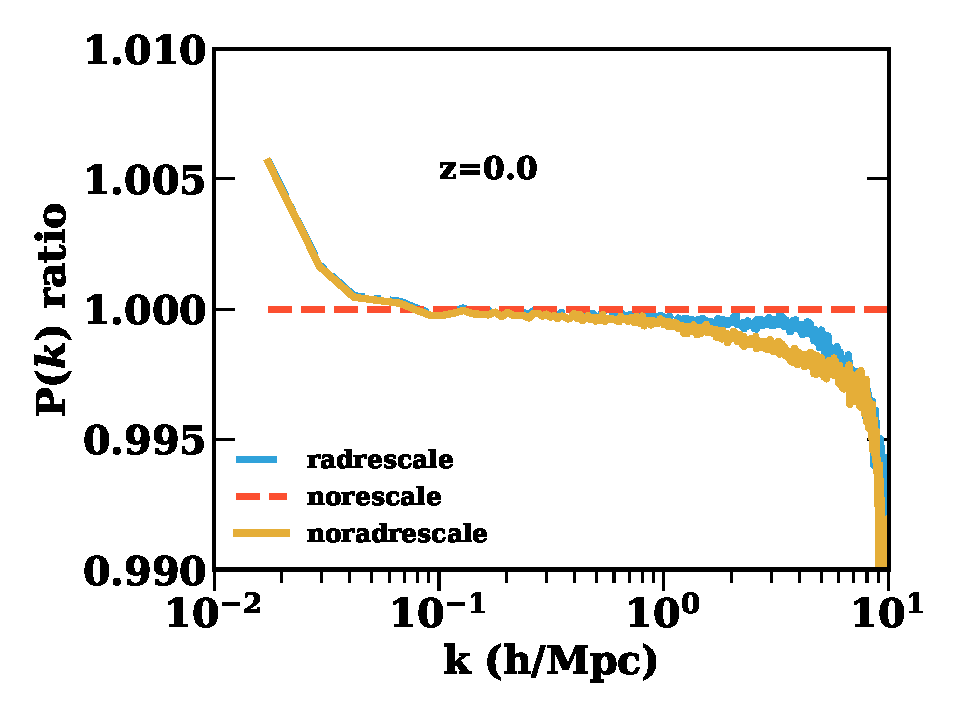
\includegraphics[width=0.45\textwidth]{icplots/pks_rel-1.pdf}
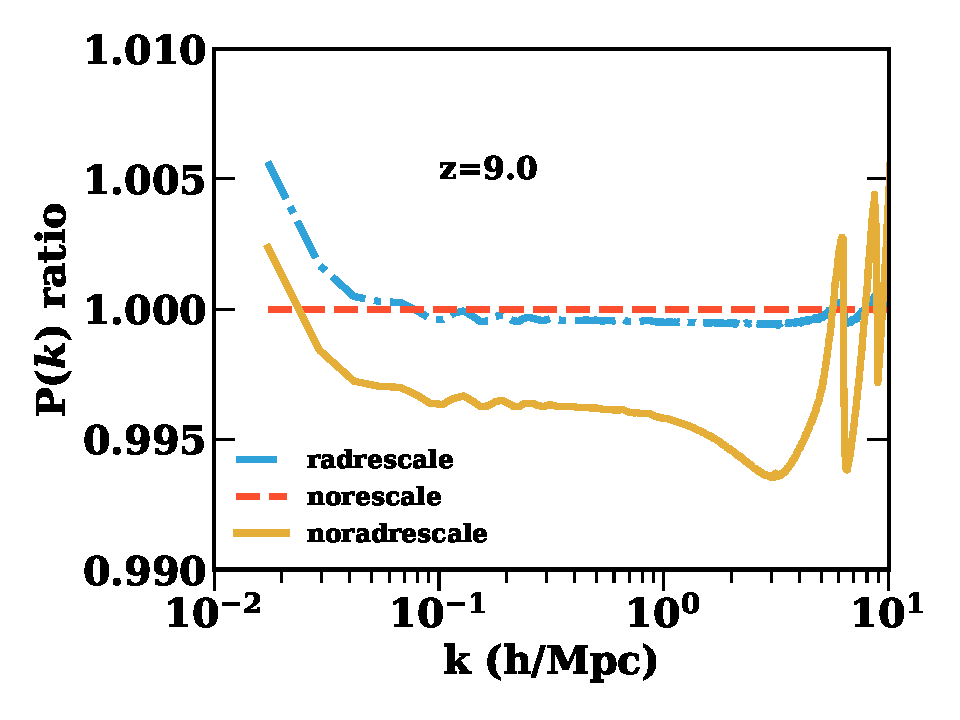
\includegraphics[width=0.45\textwidth]{icplots/pks_rel-0_1.pdf}
% \includegraphics[width=0.45\textwidth]{icplots/pks_camb-1.pdf}
  \caption{The ratio between matter power spectra from three simulations with different initial conditions.
  These are initialized respectively using the $z=99$ (norescale) transfer function,
  the scaled $z=0$ transfer function (radrescale), and the $z=0$ transfer function
  scaled and evolved neglecting radiation density (noradrescale). Power spectra are normalised to the norescale simulation.
  (Left) At $z=0$. (Right) At $z=9$.}
  \label{fig:rescaling}
\end{figure*}

In this Appendix, we detail improvements to the accuracy of our simulation initial conditions, generated using S-GenIC \footnote{\url{https://github.com/sbird/S-GenIC}}, since \cite{AHB}.
Following Lagrangian perturbation theory \citep{Zeldovich_1970, Scoccimarro_1998},
the particle velocities and displacements are related by:
\begin{equation}
v(k) = a H(a) \frac{d \log D(a)}{d \log a} \delta(k)\,.
\label{eq:vel_prefac}
\end{equation}
$D(a)$ is the linear growth function and $H = \dot{a}/a$ the Hubble function.

In \cite{AHB}, the Hubble function used in Eq.~\ref{eq:vel_prefac}
neglected radiation density. Furthermore, following \cite{Bouchet:1995}, we
approximated the derivative of the linear growth function, $\frac{d \log D(a)}{d \log a}$, by
\begin{equation}
\frac{d \log D(a)}{d \log a} \approx \left(\frac{\Omega_M a^{-3}}{\Omega_M  a^{-3} + \Omega_L}\right)^{0.6}\,.
\end{equation}
This approximation is valid in matter domination, but again neglects the radiation density,
which becomes non-negligible at $z > 50$. Both of these approximations are especially notable
when simulating massive neutrinos, because at high redshift neutrinos are slightly relativistic,
and thus the background density depends slightly on the neutrino mass. In practice the error
induced by each approximation partially cancels, leaving an under-estimation of the effect of
massive neutrinos on structure formation by $\sim 2 \%$, visible in, for example,
Figure 4 of \cite{AHB}\footnote{We thank Francisco Villaescusa-Navarro for first pointing these problems out to us.}

In the simulations presented here we use both the full Hubble function
and obtain $\frac{d \log D(a)}{d \log a}$ by numerically solving
the linear growth equation \citep{Peebles:1993}:
\begin{equation}
\frac{d}{da}\left(a^3 H(a) \frac{d D(a)}{da}\right) - \frac{3}{2} \frac{H_0^2\,D(a)}{a^2 H(a)} \left(\Omega_\mathrm{CDM} + \Omega_\mathrm{b}\right)= 0\,.
\end{equation}
The initial conditions for this differential equation are set at $z \gg 100$ corresponding
to the growing mode in a matter-radiation universe \citep{Groth:1975}:
\begin{equation}
  D(a_i) = \Omega_\mathrm{R} + \Omega_\nu + \frac{3}{2} \left(\Omega_\mathrm{CDM} + \Omega_\mathrm{b}\right) a_i\,.
\end{equation}
The above is appropriate for our simulations, because our simulation box size is smaller than the neutrino free-streaming scale at our initial redshift, and thus neutrinos do not cluster. For simulations which are on larger scales or start at much later redshift it would be necessary to incorporate the full scale-dependent growth rate, as in \cite{Zennaro_2017} or \cite{OLeary_2012}. \yah{I don't understand, why not just take the time derivative of CAMB's output??} \spb{Because then I would have to do two FFTs in the IC generator...it is totally doable, I just haven't gotten around to it yet. I can probably implement it by the time this is refereed.}

Our initial conditions are generated using the CAMB total matter transfer
function at $z=99$. An alternative is to generate initial conditions
using the $z=0$ transfer function, scaled to the initial redshift by the
linear growth function, $D(z_\mathrm{ic})$. This can
be used to account for background radiation density, if radiation is not included
in the background evolution, or for radiation perturbations and other relativistic
effects on the scale of the horizon at $z=99$ \citep{Zennaro_2017}.

Figure \ref{fig:rescaling} shows the differences in power spectra
produced with the $z=99$ transfer function, the
scaled $z=0$ transfer function, and the $z=0$ transfer function
scaled and evolved neglecting radiation density at $z=0$ and $z=9$.
For our scales of interest, these differences are small.
The largest differences occur at $z=9$ in the simulation which neglects
background radiation density, producing a change of half a percent in
the high redshift growth rate. Although this effect is small, we nevertheless suggest that simulations
which use scaled $z=0$ transfer functions still include radiation in the background.
We use the $z=99$ transfer function as it is practically and conceptually simple,
whereas the linear scaling is complex in the presence of massive neutrinos.

\label{lastpage}

\bibliography{neutrinos}

\end{document}
